\chapter{Evaluation\label{chap:evaluation}}

Many methods were used to evaluate the implementations, which can be split up into ``opaque box'' and ``clear box'' methods. One method combines a ``opaque box'' and ``clear box'' method which makes the method a bit of both. These methods and their category of either ``opaque box'' or ``clear box'' have been detailed in the Venn diagram shown in  Figure~\ref{fig:evalaution-venn-diagram}.

\begin{figure}[h]
    \centering
    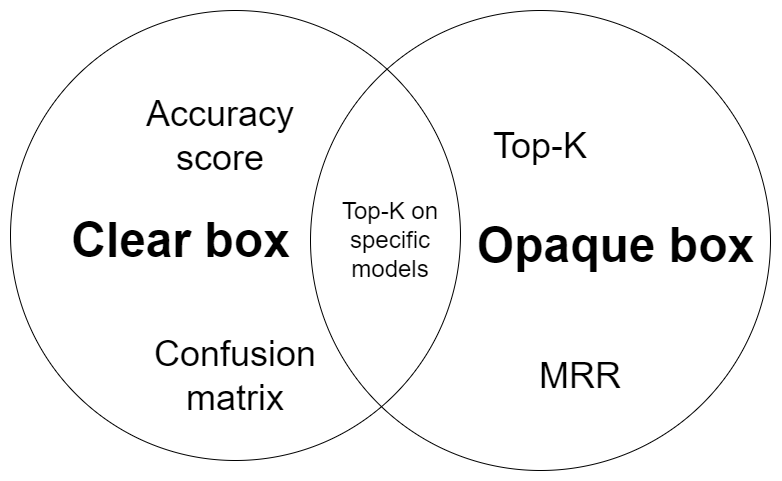
\includegraphics[scale=0.3]{images/evaluation-venn.png}
    \caption[Evaluation methods grouped by clear and opaque box in a Venn diagram.]{Evaluation methods grouped by clear and opaque box in a Venn diagram. MRR stands for Mean Reciprocal Rank.}
    \label{fig:evalaution-venn-diagram}
\end{figure}

The opaque box methods are ones which do not have access to the system except for the inputs and outputs, whereas, the clear box evaluation methods have access to the internals.

The opaque box methods have the advantage of not being implementation specific, which means that they can be compared against a variety of other implementations as long as the output (the recommended reviewers) are similar. The score generated for an implementation that is not run can be compared easily to implementations that were tested on the MediaWiki project.

Implementations from previous research were focused on other projects and as such do not directly relate to the MediaWiki project. However, the implementations created here are compared to previous work to give a rough indication of how well the implementations perform against implementations built by other projects.

This evaluation also discusses the perceived accuracy of the recommendations using our knowledge about who is best to be added to a change. This is also carried out so that screenshots of the output of the implementations can be shown in the report.

\section{Metrics and Experiment Setup}

The opaque box methods used to evaluate here are also used in other research that implements reviewer recommender systems. This is done so that the implementations here can be compared to previous research:
\begin{itemize}
    \item Top-k accuracy \citep[p. 939]{6606642} \citep[p. 506]{9240650} \citep[p. 147]{7081824}
    \item Mean Reciprocal Rank (MRR) \citep[p. 147]{7081824} \citep[p. 506]{9240650} \citep[p. 536]{7328331}
\end{itemize}

Clear box evaluation was used to compare the different approaches to the machine learning implementation. Specifically, whether the repository-specific models provided a statistically significant benefit over the generic model trained on all repositories.

If the results for the metrics are poor based on comparisons to previous work, the implementation parameters and other code changes were used to attempt to improve the solution.

To make the evaluation process easier, a script was used to produce a representative sample of the repositories. This script randomly selected repositories from two groups that were created by splitting the list of repositories at the median where the list was ordered by the number of changes in the test dataset for that repository. This significantly reduced the number of repositories being evaluated and made it possible to evaluate the neural network recommender in a reasonable amount of time. To this list was added the ``mediawiki/core'' repository as this represents the most important repository in the list of repositories and also ``mediawiki/extensions/CheckUser'' as we have experience with this repository and it would make corroborating the results easier.

We experimented with two different values to be used as the x-axis value for our graph results. These were:
\begin{itemize}
    \item The number of files in the repository.
    \item The number of changes in the test and training dataset for each repository.
\end{itemize}

The number of files in the repository was generated using git's ``ls-files'' command that lists the files in the current working tree \cite{git:ls-files}. The lines are then counted and stored for later inspection. The number of changes in the test and training dataset was easily calculated by opening it and counting the data for each repository.

Some statistics were generated for the number of files in each repository and the number of changes in the training and testing dataset, as shown in Table~\ref{table:files-vs-changes-for-x-value}.
\begin{table}[h]
\begin{center}
\begin{tabular}{@{}c c c@{}} 
\hline
\textbf{Statistic} & Number of files & Number of changes \\
\hline
Minimum & 19 & 10 \\
Maximum & 424290 & 1124 \\
Mode & 19 & 10 \\
Median & 2187 & 24 \\
10th percentile & 747 & 11 \\
90th percentile & 21093 & 105 \\
\hline
\end{tabular}
\end{center}
\caption{
\label{table:files-vs-changes-for-x-value}Comparison of statistics for the number of files and the number of changes in the training and testing dataset.}
\end{table}

\label{paragraph:mediawiki-core-being-large-in-file-count}The file counts over the repositories selected were mostly at a reasonable number, but a few repositories such as ``mediawiki/core'' (which has the maximum file count size) make the maximum and 90th percentile very large. The training and testing dataset covered a much smaller range and the median and mode were much closer together suggesting that the data is more normally distributed than the number of files.

The number of files is likely affected by translation files, as each translation has a separate JSON file and there are around 450 languages that are supported by MediaWiki \citepmediawiki{mediawiki:names-php}. However, this has not been investigated as languages that have no translations from English do not have an associated JSON file, so subtracting 450 from the file count for every repository will not work in this case.

Furthermore, the number of files in a repository does not necessarily imply activity in a repository. Deprecated or old repositories that were once very active could have large file counts. Using the number of changes in the training and testing dataset is likely a good indicator of the activity levels of a repository.

Because the statistics about the number of changes for each repository from the training and testing dataset was better than the number of files, the number of changes was chosen as the value to use for the x-axis if no other value for it was appropriate for our graphs.

Three repositories that were randomly selected (namely ``mediawiki/services/ores'', ``mediawiki/tools/phan/Utils'' and ``mediawiki/extensions/FileSystemImageServer'') were removed from the randomly sampled repositories as they had too few changes in the test dataset (under 10 from all time) which made them too inactive to produce useful results.

Once the evaluation results were produced it was clear that evaluation using ``open'' and ``abandoned'' changes for the Top-k and MRR metrics was poor. This was for many reasons:
\begin{itemize}
    \item Evaluating the prediction of approvers was impossible as changes could not have any approval votes if they had the ``open'' and ``abandoned'' status as ``merged'' changes were ones that had this approval vote. This means that there would be no actual approver to compare to.
    \item The training and testing data set often contained few changes for these status types because the data collection minimised the time period but did not check for the counts of these changes. Even if changes were collected from all time, many more changes on the Gerrit system are merged than open or abandoned.
\end{itemize}

This means that only evaluation scores produced using merged changes are detailed for section~\ref{section:evaluation-top-k} and section~\ref{section:evaluation-mrr}. However, results for these change statuses are available in Appendix~\ref{appendix:detailed-results}. Also, results for the accuracy score and confusion matrix were detailed for open and abandoned changes because the models still produced predictions for each repository

If a line of best fit is appropriate, we add this to the graphs produced in this chapter. The lines of best fit were generated using numpy's \(numpy.ployfit\) that produces ``least squares polynomial fit'' \citep{numpy:polyfit}. Paired with a degree of 1 and conversion to ``[a] one-dimensional polynomial class'' \citep{numpy:poly1d}, a straight line that represents the line of best fit is generated.

This line of best fit is then used to draw conclusions about the relationship between the number of changes in the training and testing dataset (X) and the Y values. Statistics are generated for the line of best fit using \emph{scipy's linregress} which calculates a linear least-squares regression to produce a Graident, Pearson correlation coefficient and two-sided p-value \citep{scipy:linregress}. To make these conclusions clearly defined, the following hypotheses were used where the null hypothesis is rejected if the Pearson correlation coefficient is above 0.5 and the two-sided p-value is less than 0.05.
\begin{itemize}
    \item \(H_0\) (null hypothesis) - The number of changes has no effect on the metric score shown in the Y-axis values.
    \item \(H_1\) (alternative hypothesis) - The number of changes in a repository has an effect on the metric score shown in the Y-axis values.
\end{itemize}

Because the number of changes is a good indication of the activity of a repository, this also can be used to make predictions on how the activity of the repository affects the Y value.

For evaluation of the neural network implementation, the issues relating to the data being scaled should be kept in mind as discussed on page~\pageref{para:training-when-scaling-caused-issues}. While this does affect the implementation, the effect caused seems to have been the opposite of what was expected \citep{medium:importance-of-feature-scaling} as the model seemed to produce better recommendations.

\section{Top-k\label{section:evaluation-top-k}}

Both implementations were evaluated using the Top-k method. The value of Top-k can be between 1 to 0 and represents the percentage of changes that have a recommendation match the actual reviewer or approver of the change.

The equation for this method is shown below in Equation~\ref{eq:top-k} where \(C\) is the list of changes, \(k\) is an integer, \(t\) represents either ``approved'' or ``voted'' and the method \(isRecomm(C(i), t, k)\) returns 1 if the recommender implementation for the \(i\)th change produces a user who approved or reviewed the change depending on the value of \(t\). This equation is based on the Top-k equation used in \citeauthor{9240650} \citeyear{9240650} (p. 506).

\begin{equation} \label{eq:top-k}
topk(C, t, k) = \frac{\sum_{i=0}^{|C|} isRecomm(C(i),t,k)}{|C|}
\end{equation}
\hspace{0.25cm}

The \(isRecomm(C(i), t, k)\) function is approximated by the pseudo-code shown in Algorithm~\ref{alg:isRecomm}. The function \(recommendations\_for\_change\) gets the recommendations for users who are expected to either vote or approve depending on the value in \(type\) for the \(change\). The result of \(topk(C, t, k)\) is stored for later inspection.

\hspace{0.25cm}

\begin{algorithm}[H]
	\Fn{isRecomm (change, type, k)} {
            $sanitised\_change \gets remove\_reviewer\_info\_from\_change$ $(change)$\;
            $recommendations \gets recommendations\_for\_change$ $(sanitised\_change, type)$\;
            $top\_k\_recommendations \gets get\_top\_k\_recommendations$ $(recommendations, k)$\;
            \eIf{$type = voted$}{
                $actual\_reviewers \gets get\_actual\_voters$ $(change)$\;
            }{
                $actual\_reviewers \gets get\_actual\_approvers$ $(change)$\;
            }
            \ForEach{$\{recommendation\} \in top\_k\_recommendations$} {
                \If{$recommendation \in actual\_reviewers$} {
                    \Return 1\;
                }
            }
            \Return 0\;
	}
	\caption
	{\label{alg:isRecomm}isRecomm function.}
\end{algorithm}

\hspace{0.25cm}
\label{para:evaluation-top-k-only-using-merged}To perform the evaluation, we decided to only analyse the Top-k scores generated for the changes that have been merged. This is because the method of evaluation relies on knowing the votes that have been given to a change and then comparing these to the predictions. For open and abandoned changes the number of code review votes was small, which led to the results being particularly poor. For the rule-based recommender, the Top-k scores for open and abandoned changes are detailed in Appendix~\ref{appendix:detailed-results} so that this can be seen. This was not done for the neural network recommendation method as the scores were similarly poor and therefore not worth detailing. However, these results are available in the JSON results files generated that have been included in the submission of the code. \williamnote{TODO: Actually make sure that happens.}

\subsection{Rule Based Implementation\label{section:rule-based-top-k-eval}}

For the rule based recommender, the top-k evaluation method was performed multiple times with each run having a unique unique combination of the parameters to the function \(topk(C, t, k)\):
\begin{itemize}
    \item \(t\) - The recommendation is asked to produce recommendations for users who would vote on the change or users who would approve the change.
    \item \(k\) - The values of k processed are 1, 3, 5, and 10.
\end{itemize}

The full Top-k scores (including those for ``open'' and ``abandoned'' changes) for the rule based recommender are available in Appendix~\ref{appendix:detailed-results}. \williamnote{Reference specific table, not the appendix?}\rcnote{You can reference both.}. A selection of the results in table form for changes that are ``merged'' are shown here for reference in Table~\ref{table:top-k-voted} and Table~\ref{table:top-k-approved}.

\williamnote{TODO: Find the values which are exactly 0 and see if there is a finer floating point representation. For the result tables. Done for pearson / gradient tables.}

\begin{table}[H]
\begin{center}
\begin{tabular}{@{}c c c c c@{}} 
\hline
    \textbf{Repository} &
    \multicolumn{4}{c}{\textbf{Voted Top-k}} \\
      & {Top-1} & {Top-3} & {Top-5} & {Top-10} \\
      \hline
mediawiki/extensions/CheckUser & 0.307 & \textbf{0.4} & \textbf{0.433} & \textbf{0.447} \\
mediawiki/extensions/SecureHTML & 0.007 & 0.02 & 0.053 & 0.093 \\
mediawiki/extensions/ShoutWikiAds & 0.02 & 0.02 & 0.02 & 0.02 \\
mediawiki/extensions/BlueSpiceInsertFile & 0 & 0 & 0 & 0.007 \\
mediawiki/extensions/MassMessage & 0.033 & 0.087 & 0.107 & 0.14 \\
mediawiki/extensions/CentralAuth & 0.033 & 0.047 & 0.087 & 0.1 \\
mediawiki/extensions/Workflows & 0.013 & 0.06 & 0.06 & 0.1 \\
mediawiki/core & 0.08 & 0.2 & 0.3 & \textbf{0.44} \\
mediawiki/extensions/GrowthExperiments & \textbf{0.44} & \textbf{0.74} & \textbf{0.76} & \textbf{0.767} \\
mediawiki/extensions/Translate & 0.227 & \textbf{0.46} & \textbf{0.533} & \textbf{0.553} \\
mediawiki/skins/Vector & 0.167 & 0.38 & \textbf{0.413} & \textbf{0.547} \\
\hline
\end{tabular}
\end{center}
\caption{\label{table:top-k-voted}Top-k scores where k is 1, 3, 5 or 10 for predicting users who have voted on a change.}
\end{table}

\begin{table}[H]
\begin{center}
\hspace{0.25cm}
\begin{tabular}{@{}c c c c c@{}} 
 \hline
    \textbf{Repository} &
    \multicolumn{4}{c}{\textbf{Approved Top-k}} \\
      & {Top-1} & {Top-3} & {Top-5} & {Top-10} \\
      \hline
mediawiki/extensions/CheckUser & 0.3 & 0.387 & \textbf{0.427} & \textbf{0.44} \\
mediawiki/extensions/SecureHTML & 0.007 & 0.013 & 0.047 & 0.08 \\
mediawiki/extensions/ShoutWikiAds & 0.02 & 0.02 & 0.02 & 0.02 \\
mediawiki/extensions/BlueSpiceInsertFile & 0 & 0 & 0 & 0.007 \\
mediawiki/extensions/MassMessage & 0.027 & 0.08 & 0.1 & 0.133 \\
mediawiki/extensions/CentralAuth & 0.033 & 0.047 & 0.087 & 0.1 \\
mediawiki/extensions/Workflows & 0.013 & 0.06 & 0.06 & 0.1 \\
mediawiki/core & 0.06 & 0.187 & 0.28 & \textbf{0.413} \\
mediawiki/extensions/GrowthExperiments & 0.393 & \textbf{0.713} & \textbf{0.733} & \textbf{0.733} \\
mediawiki/extensions/Translate & 0.2 & \textbf{0.42} & \textbf{0.513} & \textbf{0.533} \\
mediawiki/skins/Vector & 0.14 & 0.36 & 0.393 & \textbf{0.527} \\
\hline
\end{tabular}
\end{center}
\caption{\label{table:top-k-approved}Top-k scores where k is 1, 3, 5 or 10 for predicting users who have approved a change.}
\end{table}

As can be seen by the selection of the results above the rule based recommender Top-k scores vary largely between repository and the number of recommendations (\(k\)). The results above \(0.4\) are highlighted in bold for easier reference.

The rule based recommender performs better at predicting users that have voted on changes than approved, as can be seen by comparing the results for each repository in Tables~\ref{table:top-k-voted} and \ref{table:top-k-voted}.

``mediawiki/extensions/GrowthExperiments'', which is a WMF wiki deployed extension used by the WMF Growth team to evaluate tools they are working on \citepmediawiki{mediawiki:growth-experiments}, received the best Top-k scores across the board with accuracy being very good in both recommending users who actually voted and users who actually approved for k of 3 and above. This suggests that the rule based implementation would work well running live on MediaWiki if just targeted this extension.

``mediawiki/core'', ``mediawiki/skins/Vector'', ``mediawiki/extensions/Translate'' and ``mediawiki/extensions/CheckUser'' also perform well. These four repositories represent critical parts of the MediaWiki project with the core repository being the base install, the ``Vector'' skin being the default skin for MediaWiki and is the default look of Wikipedia for logged in and out users \citepmediawiki{mediawiki:vector}, the ``Translate'' extension being used to translate MediaWiki on TranslateWiki.net\footnote{\url{https://translatewiki.net}. Accessed 13 May 2023} \citepmediawiki{mediawiki:translate} and ``CheckUser'' being used to combat abuse \citep[p. 158]{10.1145/2030376.2030394}.

The results in Tables~\ref{table:top-k-voted} and \ref{table:top-k-approved} suggests that for the full list of repositories being evaluated, the extension activity may have an effect on the Top-k score. To investigate this graphs are produced of change counts in the training and testing data set against the Top-k scores.

To find an appropriate set of values for each repository to be used as the X axis value, the number of files and number of changes in the training and testing dataset were both initially used to produce graphs. As shown below in Figure~\ref{fig:rule-based-top-k-files-vs-changes-approved} and Figure~\ref{fig:rule-based-top-k-files-vs-changes-voted}, using the file counts as the value for X led to much more variation of Top-k value between neighbouring data points. As such using the number of changes in the training and testing dataset is a better way to visualise the data, and has been used for the Top-k result graphs.

\begin{figure}[H]%
    \centering
    \subfloat[\centering Using change counts as X axis.]{{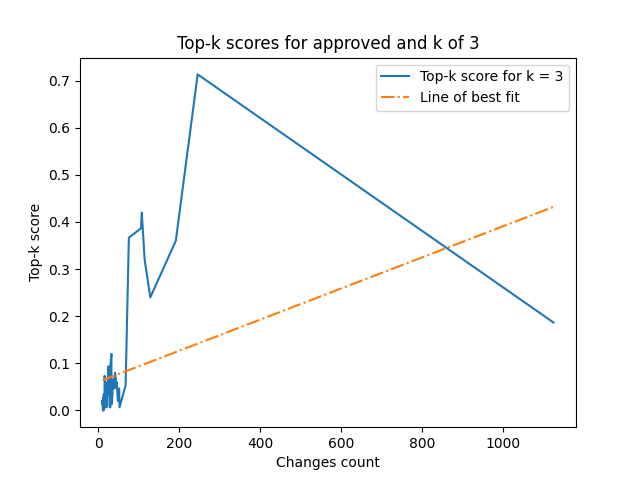
\includegraphics[height=5cm]{images/graphs/rule-based-top-k-approved-k-3.png} }}%
    \subfloat[\centering Using file counts as X axis.]{{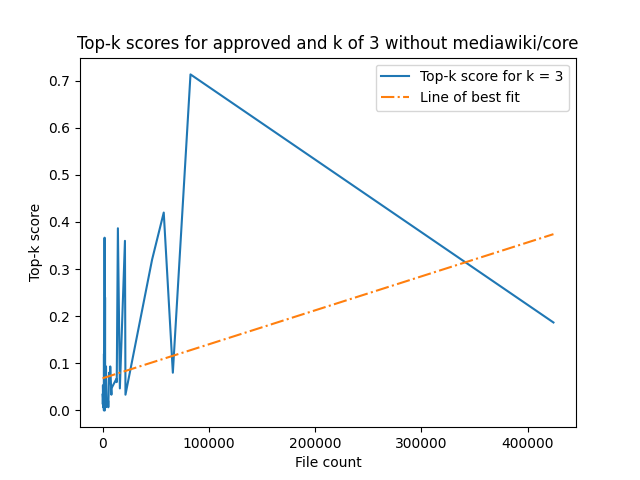
\includegraphics[height=5cm]{images/graphs/rule-based-top-k-approved-k-3-files.png} }}%
    \caption{Comparison of using file counts or change counts as the x-axis values when predicting approvers where k is 3.}%
    \label{fig:rule-based-top-k-files-vs-changes-approved}%
\end{figure}

\begin{figure}[H]%
    \centering
    \subfloat[\centering Using change counts as X axis.]{{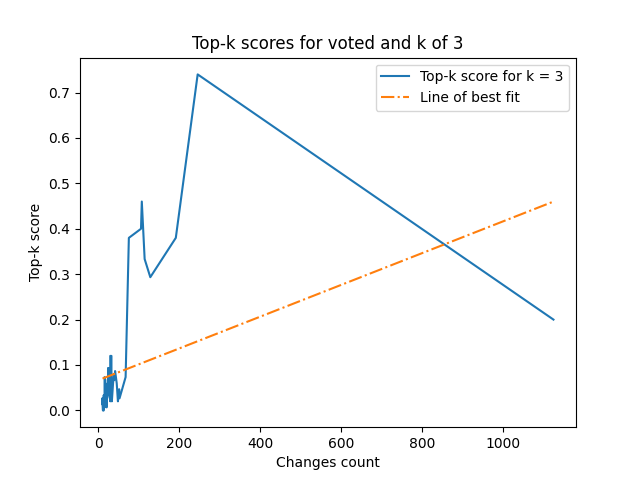
\includegraphics[height=5cm]{images/graphs/rule-based-top-k-voted-k-3.png} }}%
    \subfloat[\centering Using file counts as X axis.]{{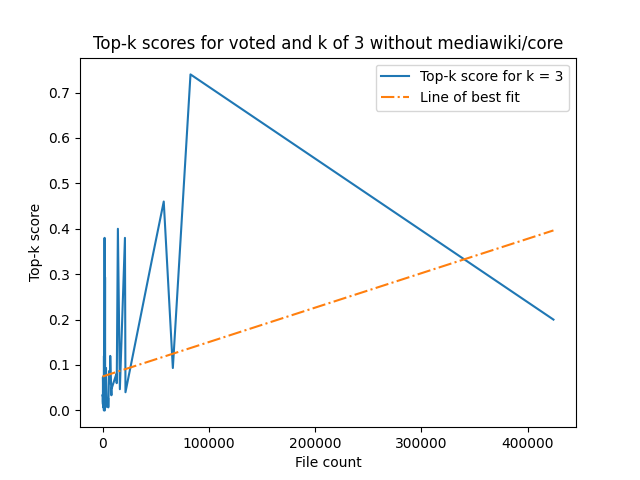
\includegraphics[height=5cm]{images/graphs/rule-based-top-k-voted-k-3-files.png} }}%
    \caption{Comparison of using file counts or change counts as the x-axis values when predicting voters where k is 3.}%
    \label{fig:rule-based-top-k-files-vs-changes-voted}%
\end{figure}

The graphs in Figures~\ref{fig:rule-based-top-k-approved-k-1} and \ref{fig:rule-based-top-k-voted-k-10} below show the relationship between the number of changes for the repository in the training and testing dataset (X) and the Top-k score (Y). The graphs labelled \emph{(a)} include every repository selected for evaluation, whereas, the graphs labelled \emph{(b)} include every repository selected for evaluation except ``mediawiki/core''.

The graphs labelled \emph{(b)} were produced as it was noticed that the repository with the largest change count (``mediawiki/core'') did not meet the expected trend of increasing Top-k score against changes count. The author posits that because this repository is so abnormally large based on file count (as discussed above on page~\pageref{paragraph:mediawiki-core-being-large-in-file-count}), the rule based system performs worse because it relies on data points generated per repository and cannot adapt itself per repository.

Graphs where k is 3 and 5 look similar to the graphs where k is 10. Therefore to save space they are shown in Appendix~\ref{appendix:detailed-results} as Figures~\ref{fig:rule-based-top-k-approved-k-3-appendix-c} and \ref{fig:rule-based-top-k-approved-k-5-appendix-c}.

\begin{figure}[H]%
    \centering
    \subfloat[\centering All repositories.]{{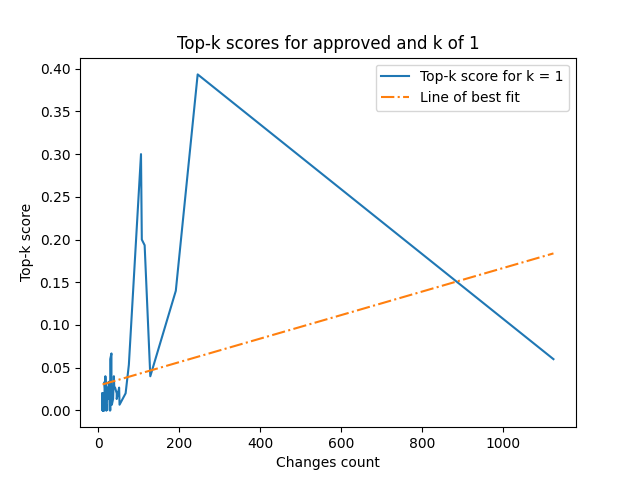
\includegraphics[height=5cm]{images/graphs/rule-based-top-k-approved-k-1.png} }}%
    \subfloat[\centering Without mediawiki/core.]{{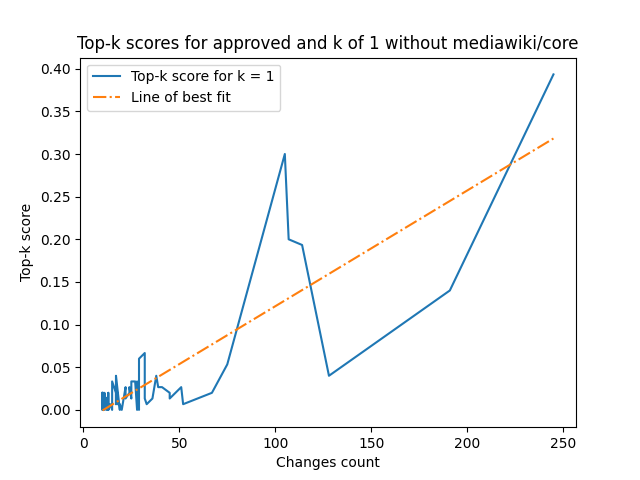
\includegraphics[height=5cm]{images/graphs/rule-based-top-k-approved-k-1-no-core.png} }}%
    \caption{Rule based recommender Top-k score for correctly predicting approvers where k is 1.}%
    \label{fig:rule-based-top-k-approved-k-1}%
\end{figure}

\begin{figure}[H]%
    \centering
    \subfloat[\centering All repositories.]{{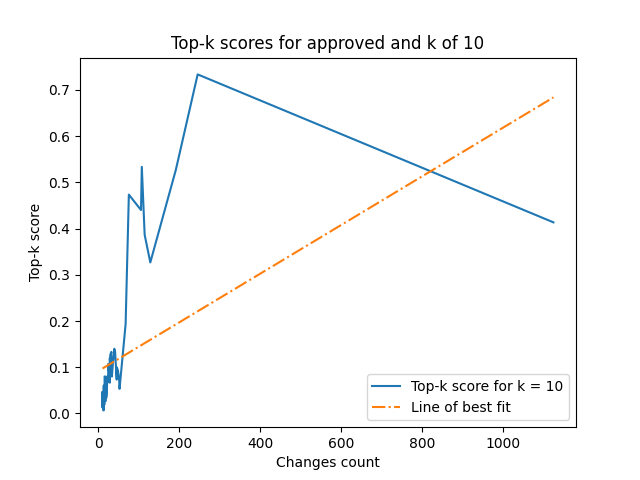
\includegraphics[height=5cm]{images/graphs/rule-based-top-k-approved-k-10.png} }}%
    \subfloat[\centering Without mediawiki/core.]{{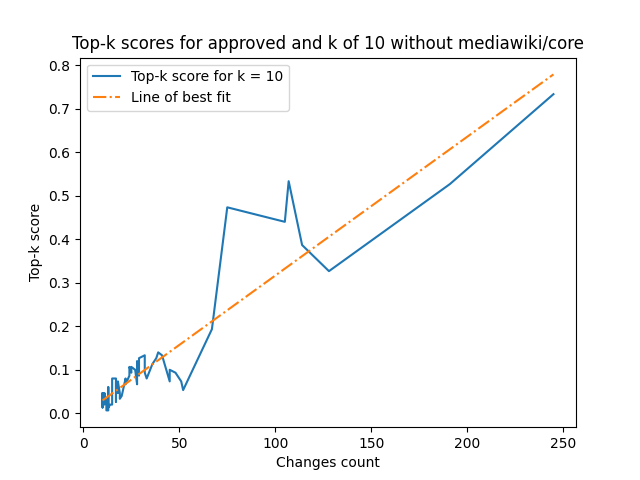
\includegraphics[height=5cm]{images/graphs/rule-based-top-k-approved-k-10-no-core.png} }}%
    \caption{Rule based recommender Top-k score for correctly predicting approvers where k is 10.}%
    \label{fig:rule-based-top-k-approved-k-10}%
\end{figure}

As can be seen in Figures~\ref{fig:rule-based-top-k-approved-k-1} and \ref{fig:rule-based-top-k-approved-k-10}, a visual inspection of the line of best fit shows that the the Top-k score for predicting users who will approve a change improves with the number of changes. This still is a noticeable increase even when including the outlier repository ``mediawiki/core''.

To quantify this relationship the graident, pearson correlation coefficent and p-value associated with the line of best fit for each graph was produced and is shown in Table~\ref{table:top-k-line-of-best-fit-for-approved}.

\begin{table}[H]
    \centering
    \begin{tabular}{@{}c c c c c@{}} 
    \hline
    \textbf{Graph label} & \textbf{K value} & \textbf{Gradient} & \textbf{Pearson correlation coefficient} & \textbf{two-sided p-value} \\
    \hline
Figure~\ref{fig:rule-based-top-k-approved-k-1} \emph{(a)} & 1 & 0.000138 & 0.287 & 0.0251 \\
Figure~\ref{fig:rule-based-top-k-approved-k-1} \emph{(b)} & 1 & 0.00136 & 0.833 & 1.56e-16 \\
Figure~\ref{fig:rule-based-top-k-approved-k-3-appendix-c} \emph{(a)} & 3 & 0.00033 & 0.369 & 0.0034 \\
Figure~\ref{fig:rule-based-top-k-approved-k-3-appendix-c} \emph{(b)} & 3 & 0.00275 & 0.91 & 8.12e-24 \\
Figure~\ref{fig:rule-based-top-k-approved-k-5-appendix-c} \emph{(a)} & 5 & 0.000414 & 0.421 & 0.00072 \\
Figure~\ref{fig:rule-based-top-k-approved-k-5-appendix-c} \emph{(b)} & 5 & 0.00297 & 0.902 & 8.38e-23 \\
Figure~\ref{fig:rule-based-top-k-approved-k-10} \emph{(a)} & 10 & 0.000526 & 0.506 & 3.23e-05 \\
Figure~\ref{fig:rule-based-top-k-approved-k-10} \emph{(b)} & 10 & 0.00319 & 0.932 & 3.01e-27 \\
    \hline
    \end{tabular}
    \caption{Gradient, Pearson correlation coefficient and p-value for the line of best fit for graphs in Figures~\ref{fig:rule-based-top-k-approved-k-1}, \ref{fig:rule-based-top-k-approved-k-3-appendix-c}, \ref{fig:rule-based-top-k-approved-k-5-appendix-c}, and \ref{fig:rule-based-top-k-approved-k-10}.}
    \label{table:top-k-line-of-best-fit-for-approved}
\end{table}

Next graphs are created for how well the rule based recommender predicts users who actually voted on the change. These are shown in Figures~\ref{fig:rule-based-top-k-voted-k-1} and \ref{fig:rule-based-top-k-voted-k-10} for k equal to 1 and 10 respectively. Graphs for k equal to 3 and 5 are shown in Appendix~\ref{appendix:detailed-results} as they were similar to the graph for k equal to 10.

\begin{figure}[H]%
    \centering
    \subfloat[\centering All repositories selected for evaluation.]{{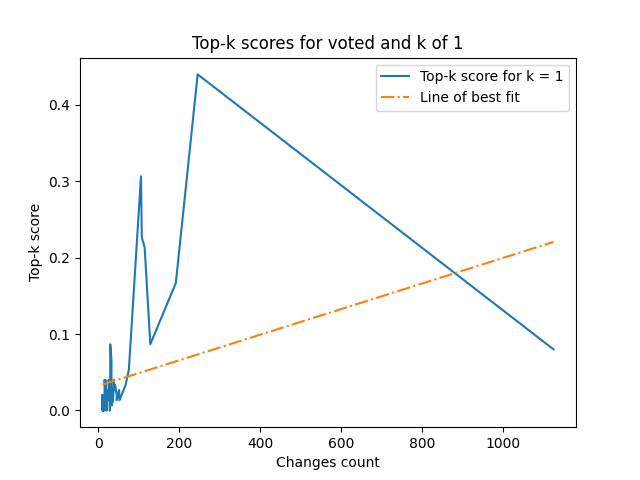
\includegraphics[height=5cm]{images/graphs/rule-based-top-k-voted-k-1.png} }}%
    \subfloat[\centering Without mediawiki/core.]{{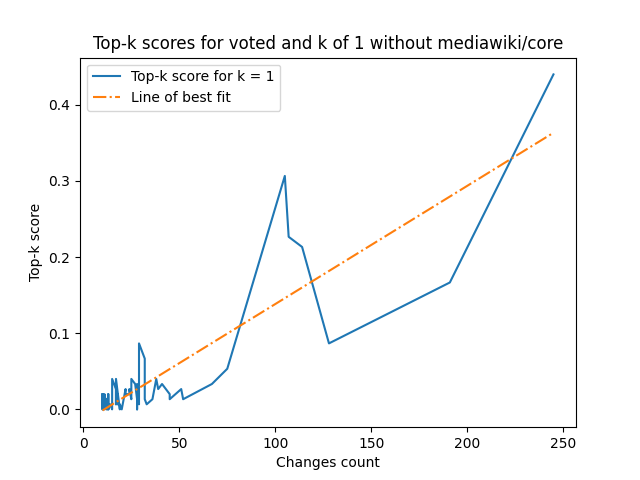
\includegraphics[height=5cm]{images/graphs/rule-based-top-k-voted-k-1-no-core.png} }}%
    \caption{Rule based recommender Top-k score for correctly predicting voters where k is 1.}%
    \label{fig:rule-based-top-k-voted-k-1}%
\end{figure}

\begin{figure}[H]%
    \centering
    \subfloat[\centering All repositories.]{{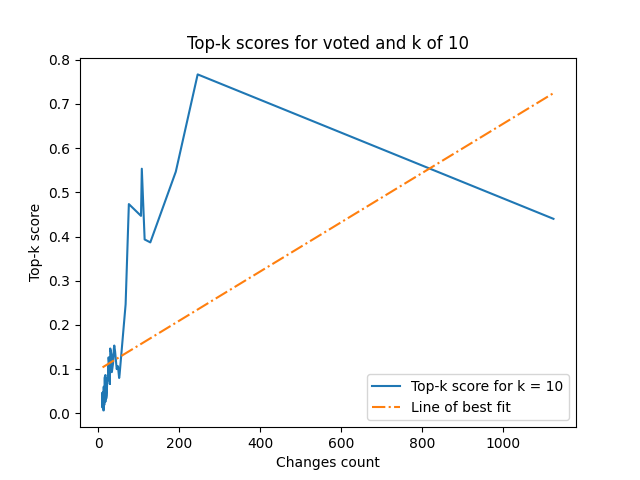
\includegraphics[height=5cm]{images/graphs/rule-based-top-k-voted-k-10.png} }}%
    \subfloat[\centering Without mediawiki/core.]{{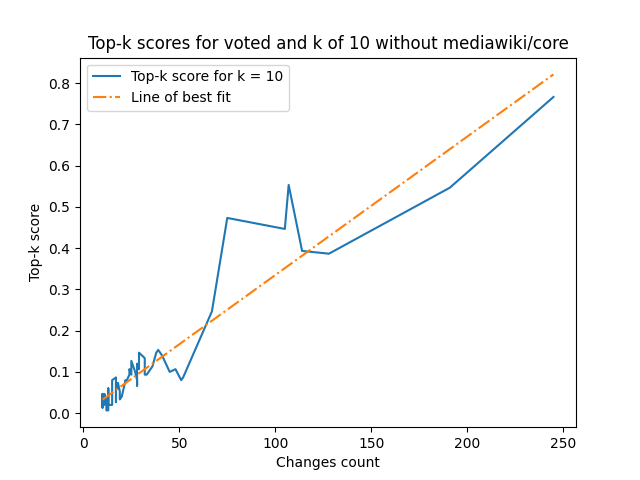
\includegraphics[height=5cm]{images/graphs/rule-based-top-k-voted-k-10-no-core.png} }}%
    \caption{Rule based recommender Top-k score for correctly predicting voters where k is 10.}%
    \label{fig:rule-based-top-k-voted-k-10}%
\end{figure}

Similar to the results for predicting approvers, the graphs all visually seem to suggest that the rule based recommender is better at recommending users who would vote on the change when the activity of the repository is increased. To quantify this, Table~\ref{table:top-k-line-of-best-fit-for-voted} details the gradient, pearson correlation coefficient and two-sided p-values for graphs in Figures~\ref{fig:rule-based-top-k-voted-k-1}, \ref{fig:rule-based-top-k-voted-k-3-appendix-c}, \ref{fig:rule-based-top-k-voted-k-5-appendix-c} and \ref{fig:rule-based-top-k-voted-k-10}.

\begin{table}[H]
    \centering
    \begin{tabular}{@{}c c c c c@{}} 
    \hline
    \textbf{Graph label} & \textbf{K value} & \textbf{Gradient} & \textbf{Pearson correlation coefficient} & \textbf{two-sided p-value} \\
    \hline
Figure~\ref{fig:rule-based-top-k-voted-k-1} \emph{(a)} & 1 & 0.000168 & 0.317 & 0.013 \\
Figure~\ref{fig:rule-based-top-k-voted-k-1} \emph{(b)} & 1 & 0.00155 & 0.865 & 5.02e-19 \\
Figure~\ref{fig:rule-based-top-k-voted-k-3-appendix-c} \emph{(a)} & 3 & 0.00035 & 0.373 & 0.00311 \\
Figure~\ref{fig:rule-based-top-k-voted-k-3-appendix-c} \emph{(b)} & 3 & 0.00291 & 0.918 & 5.81e-25 \\
Figure~\ref{fig:rule-based-top-k-voted-k-5-appendix-c} \emph{(a)} & 5 & 0.000438 & 0.43 & 0.000537 \\
Figure~\ref{fig:rule-based-top-k-voted-k-5-appendix-c} \emph{(b)} & 5 & 0.00312 & 0.915 & 1.46e-24 \\
Figure~\ref{fig:rule-based-top-k-voted-k-10} \emph{(a)} & 10 & 0.000557 & 0.513 & 2.34e-05 \\
Figure~\ref{fig:rule-based-top-k-voted-k-10} \emph{(b)} & 10 & 0.00336 & 0.943 & 2.54e-29 \\
    \hline
    \end{tabular}
    \caption{Gradient, Pearson correlation coefficient and p-value for the line of best fit for graphs in Figures~\ref{fig:rule-based-top-k-voted-k-1}, \ref{fig:rule-based-top-k-voted-k-3-appendix-c}, \ref{fig:rule-based-top-k-voted-k-5-appendix-c}, and \ref{fig:rule-based-top-k-voted-k-10}.}
    \label{table:top-k-line-of-best-fit-for-voted}
\end{table}

As can be seen in Table~\ref{table:top-k-line-of-best-fit-for-approved} and \ref{table:top-k-line-of-best-fit-for-voted} all graphs, including ones that include ``mediawiki/core'', have a two-sided p-value associated with their line of best fit that is less than 0.05. However, only graphs that do not include mediawiki/core have a Pearson correlation coefficient greater than 0.5. This therefore gives strong evidence to reject \(H_0\) for the rule based recommender and say that the rule based recommender works better the more changes there are (and therefore better for more active repositories).

\subsection{Neural Network Implementation}

The MLP classifier (neural network) implementation was also evaluated using the Top-k metric. This was done so that the implementations could be compared to each other in section~\ref{section:comparing-recommendations}. The representative sample of repositories shown in tables here are also used in this section to make it easier to directly compare this section and section~\ref{section:rule-based-top-k-eval} to make it easy to compare the results to the rule based recommender.

Unlike the rule based recommender, there are a few more parameters to the function $recommendations\_for\_change$ detailed in Algorithm~\ref{alg:isRecomm}. When performing the MLP Top-k evaluation the function is passed the model type and selection mode, where the model type is one of the types detailed in Table~\ref{table:mlp-model-types} and the selection mode is one of the ones detailed on page~\ref{para:selection-mode-neural-network}. To allow this the top-k function is passed these extra arguments for use only in calling the $recommendations\_for\_change$ function and so is known as \(topk(C, t, k, s, m)\) where \(s\) represents the selection mode and \(m\) represents the model type.

The Top-k evaluation method detailed in Equation~\ref{eq:top-k} was performed multiple times with the following unique combination of parameters to the function \(topk(C, t, k, s, m)\):
\begin{itemize}
    \item \(s\) - The technique used for ordering which is one of ``random'', ``semi-random'' or ``in-order'' as described on page~\ref{para:selection-mode-neural-network}
    \item \(m\) - The type of model used to make the recommendation (one of the ones in Table~\ref{table:mlp-model-types})
    \item \(t\) - The recommendation is asked to produce predicted voters or approvers depending on the value of t.
    \item \(k\) - The values of k processed at 1, 3, 5 and 10.
\end{itemize}

\subsubsection{Top-k on specific models}
The model types that were evaluated were the ones mentioned in Table~\ref{table:mlp-model-types}. However, because of the same issues detailed on page~\pageref{para:evaluation-top-k-only-using-merged} apply to the models for the `abandoned' and `open' models. Specifically, not enough repositories had this type of model to make analysis possible. The graphs, such as the one in Figure~\ref{fig:top-k-why-only-merged-repo-specific-and-generic} that were produced after evaluation was complete suggested poor Top-k scores for these two model types. Therefore these models are not discussed in any detail for the Top-k evaluation other than the other model types were better.

\begin{figure}[h]%
    \centering
    \subfloat[\centering Open model]{{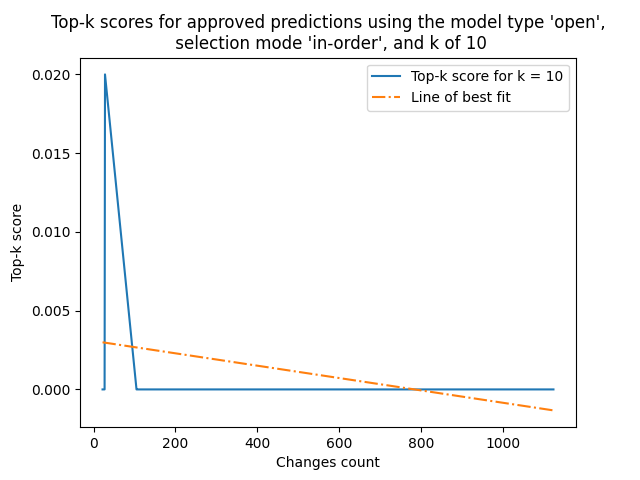
\includegraphics[height=5cm]{images/graphs/neural-network-top-k-approved-k-10-model-mode-open-selection-mode-in-order.png} }}%
    \subfloat[\centering Abandoned model]{{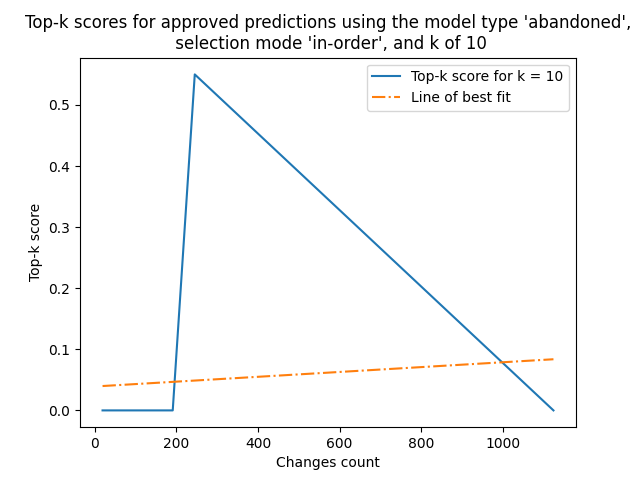
\includegraphics[height=5cm]{images/graphs/neural-network-top-k-approved-k-10-model-mode-abandoned-selection-mode-in-order.png} }}%
    \caption{Graphs detailing poor Top-k scores in general for open and abandoned model types}%
    \label{fig:top-k-why-only-merged-repo-specific-and-generic}%
\end{figure}

Although two model types are excluded, further refining of the results was needed to make it possible to discuss them in this section. To do this two representative repositories was chosen from the list of repositories selected for evaluation. These then had the Top-k scores generated for each combination of selection mode and model type, which were then tabled.

The first chosen repository, mediawiki/extensions/GrowthExperiments, had the largest Top-k score when evaluating the rule based recommender. This large Top-k score would give the neural network a better chance at producing higher Top-k scores so that the differences between each settings would be easier to see. The Top-k scores for this repository are detailed in the Tables~\ref{table:top-k-results-growth-experiements-over-combinations-approved} and \ref{table:top-k-results-growth-experiements-over-combinations-voted}.

The second repository chosen is mediawiki/extensions/MassMessage which had a relatively low Top-k score overall in the rule based recommendation but was not very low. This was added to ensure that the conclusions drawn from the first repository about the correct settings could be applied to repositories that are likely to have a poorer Top-k score. The Top-k scores for this repository are detailed in the Tables~\ref{table:top-k-results-mass-message-over-combinations-approved} and \ref{table:top-k-results-mass-message-over-combinations-voted}

\williamnote{TODO: Better captions for these tables?}
\begin{table}[H]
    \centering
    \begin{tabular}{@{}c c c c c c@{}} 
 \hline
    \textbf{Selection mode} & \textbf{Model type} &
    \multicolumn{4}{c}{\textbf{Approved Top-k}} \\
      & & {Top-1} & {Top-3} & {Top-5} & {Top-10} \\
\hline
random & generic & 0.01 & 0.02 & 0.11 & 0.17 \\
random & repo-specific & 0.07 & 0.22 & 0.33 & 0.58 \\
random & merged & 0.12 & 0.48 & 0.61 & 0.69 \\
\hline
semi-random & generic & 0.05 & 0.2 & 0.31 & 0.32 \\
semi-random & repo-specific & 0.08 & 0.4 & 0.51 & 0.58 \\
semi-random & merged & 0.25 & 0.54 & 0.66 & 0.66 \\
\hline
in-order & generic & 0.28 & 0.28 & 0.3 & 0.31 \\
in-order & repo-specific & 0.41 & 0.6 & 0.6 & 0.6 \\
in-order & merged & 0.4 & 0.66 & 0.66 & 0.66 \\
\hline
\end{tabular}
    \caption{Neural network Top-k scores for predicting approvers on the repository mediawiki/extensions/GrowthExperiments with differing model types and selection modes}
    \label{table:top-k-results-growth-experiements-over-combinations-approved}
\end{table}

\begin{table}[H]
    \centering
    \begin{tabular}{@{}c c c c c c@{}} 
 \hline
    \textbf{Selection mode} & \textbf{Model type} &
    \multicolumn{4}{c}{\textbf{Voted Top-k}} \\
      & & {Top-1} & {Top-3} & {Top-5} & {Top-10} \\
\hline
random & generic & 0.01 & 0.04 & 0.13 & 0.21 \\
random & repo-specific & 0.11 & 0.25 & 0.36 & 0.62 \\
random & merged & 0.18 & 0.54 & 0.64 & 0.73 \\
\hline
semi-random & generic & 0.05 & 0.27 & 0.36 & 0.36 \\
semi-random & repo-specific & 0.13 & 0.43 & 0.54 & 0.6 \\
semi-random & merged & 0.31 & 0.59 & 0.68 & 0.68 \\
\hline
in-order & generic & 0.34 & 0.34 & 0.35 & 0.36 \\
in-order & repo-specific & 0.44 & 0.62 & 0.62 & 0.63 \\
in-order & merged & 0.45 & 0.68 & 0.68 & 0.68 \\
\hline
\end{tabular}
    \caption{Neural network Top-k scores for predicting voters on the repository mediawiki/extensions/GrowthExperiments with differing model types and selection modes}
    \label{table:top-k-results-growth-experiements-over-combinations-voted}
\end{table}

\begin{table}[H]
    \centering
    \begin{tabular}{@{}c c c c c c@{}} 
 \hline
    \textbf{Selection mode} & \textbf{Model type} &
    \multicolumn{4}{c}{\textbf{Approved Top-k}} \\
      & & {Top-1} & {Top-3} & {Top-5} & {Top-10} \\
\hline
random & generic & 0.01 & 0.01 & 0.02 & 0.09 \\
random & repo-specific & 0.03 & 0.16 & 0.18 & 0.3 \\
random & merged & 0.03 & 0.11 & 0.14 & 0.27 \\
\hline
semi-random & generic & 0.03 & 0.1 & 0.11 & 0.11 \\
semi-random & repo-specific & 0.05 & 0.16 & 0.22 & 0.33 \\
semi-random & merged & 0.08 & 0.2 & 0.27 & 0.3 \\
\hline
in-order & generic & 0.07 & 0.09 & 0.11 & 0.11 \\
in-order & repo-specific & 0.17 & 0.25 & 0.27 & 0.31 \\
in-order & merged & 0.17 & 0.24 & 0.27 & 0.31 \\
\hline
\end{tabular}
    \caption{Neural network Top-k scores for predicting approvers on the repository mediawiki/extensions/MassMessage with differing model types and selection modes}
    \label{table:top-k-results-mass-message-over-combinations-approved}
\end{table}

\begin{table}[H]
    \centering
    \begin{tabular}{@{}c c c c c c@{}} 
 \hline
    \textbf{Selection mode} & \textbf{Model type} &
    \multicolumn{4}{c}{\textbf{Voted Top-k}} \\
      & & {Top-1} & {Top-3} & {Top-5} & {Top-10} \\
\hline
random & generic & 0.01 & 0.01 & 0.02 & 0.1 \\
random & repo-specific & 0.04 & 0.17 & 0.18 & 0.31 \\
random & merged & 0.04 & 0.14 & 0.17 & 0.27 \\
\hline
semi-random & generic & 0.04 & 0.12 & 0.13 & 0.14 \\
semi-random & repo-specific & 0.05 & 0.16 & 0.23 & 0.33 \\
semi-random & merged & 0.09 & 0.21 & 0.27 & 0.3 \\
\hline
in-order & generic & 0.08 & 0.1 & 0.13 & 0.14 \\
in-order & repo-specific & 0.17 & 0.25 & 0.28 & 0.31 \\
in-order & merged & 0.17 & 0.24 & 0.28 & 0.31 \\
\hline
\end{tabular}
    \caption{Neural network Top-k scores for predicting voters on the repository mediawiki/extensions/MassMessage with differing model types and selection modes}
    \label{table:top-k-results-mass-message-over-combinations-voted}
\end{table}

As can be seen from Tables \ref{table:top-k-results-growth-experiements-over-combinations-approved} to \ref{table:top-k-results-mass-message-over-combinations-voted}, the ``in-order`` selection mode generally produces better Top-k scores. Compared to the ``random'' selection mode, the scores are not roughly equal until k is 10 and the generic model never reaches comparable scores even at k equal to 10. Compared to the ``semi-random'' selection mode, the scores are mostly equal when once k is 5. This is likely because the maximum distance that semi-random mode allows an item to move is 5 positions, so the top of the list won't change.

\label{para:use-in-order-for-neural-network}Recommending more than 5 users at once is likely to give the user too many choices to select from, especially for newer users. As such a live implementation of the tool would likely return somewhere around 3 to 5 recommendations. This means the ``random'' selection mode is ruled out unless further improvements are made to the tool that increase the Top-k scores for this mode. Using the ``semi-random'' selection mode seems permissible as long as at least 3 users are recommended when making recommendations. For the rest of this Top-k evaluation section, the ``in-order'' selection mode is used as it produced the best Top-k scores.

Focusing in on the in-order selection mode means that we can pick from the model type. In choosing the best model type there are several things to consider other than the best Top-k score. The advantage of the generic model, as discussed in section~\ref{section:neural-network-recommender-implementation}, is that it doesn't suffer from the cold start problem for new repositories. However, for larger and established repositories using the ``repo-specific'' or ``merged'' model type should not be a problem as the data exists to make the cold start problem not applicable.

Based on the Top-k scores the worst performing model type is the ``generic'' models which suggests that when a repository has enough training data it should not use this model type to make recommendations. The ``repo-specific'' and ``merged'' model types have similar Top-k scores for the in-order selection mode, however, if using any other mode the ``merged'' model type is noticeably better. As such, this seems to suggest that the use of any of the three models in specific circumstances is not a bad idea. To make the evaluation from here easier, the ``repo-specific'' model is chosen.

\williamnote{TODO: Replace "selection mode" with "sorting mode"? Would be a better descriptor but may not be worth the effort.}

\subsubsection{Top-k on repo-specific model type and in-order selection mode}

This means that the evaluation using the Top-k method uses the ``repo-specific'' model type and ``in-order'' selection method. Tables~\ref{table:top-k-approved-neural-network} and \ref{table:top-k-voted-neural-network} detail the Top-k results from a representative sample of repositories that were used to evaluate this implementation. The full results for the ``repo-specific'' model type and ``in-order'' selection mode available in Appendix~\ref{appendix:detailed-results}.

\begin{table}[H]
\begin{center}
\begin{tabular}{@{}c c c c c@{}} 
\hline
    \textbf{Repository} &
    \multicolumn{4}{c}{\textbf{Approved Top-k}} \\
      & {Top-1} & {Top-3} & {Top-5} & {Top-10} \\
      \hline
mediawiki/extensions/CheckUser & 0.23 & 0.26 & 0.27 & 0.29 \\
mediawiki/extensions/SecureHTML & 0.01 & 0.07 & 0.09 & 0.12 \\
mediawiki/extensions/ShoutWikiAds & 0.02 & 0.02 & 0.02 & 0.02 \\
mediawiki/extensions/BlueSpiceInsertFile & 0 & 0.01 & 0.01 & 0.01 \\
mediawiki/extensions/MassMessage & 0.17 & 0.25 & 0.27 & 0.31 \\
mediawiki/extensions/CentralAuth & 0.02 & 0.02 & 0.02 & 0.02 \\
mediawiki/extensions/Workflows & 0.03 & 0.06 & 0.06 & 0.06 \\
mediawiki/core & 0.04 & 0.07 & 0.09 & 0.13 \\
mediawiki/extensions/GrowthExperiments & \textbf{0.41} & \textbf{0.6} & \textbf{0.6} & \textbf{0.6} \\
mediawiki/extensions/Translate & \textbf{0.6} & \textbf{0.74} & \textbf{0.75} & \textbf{0.77} \\
mediawiki/skins/Vector & 0 & 0.19 & 0.2 & 0.23 \\
\hline
\end{tabular}
\end{center}
\caption{\label{table:top-k-approved-neural-network}Neural network Top-k scores for predicting approvers using the ``repo-specific'' model type and ``in-order'' selection mode.}
\end{table}

\begin{table}[H]
\begin{center}
\begin{tabular}{@{}c c c c c@{}} 
\hline
    \textbf{Repository} &
    \multicolumn{4}{c}{\textbf{Voted Top-k}} \\
      & {Top-1} & {Top-3} & {Top-5} & {Top-10} \\
      \hline
mediawiki/extensions/CheckUser & 0.24 & 0.27 & 0.27 & 0.29 \\
mediawiki/extensions/SecureHTML & 0.01 & 0.07 & 0.09 & 0.13 \\
mediawiki/extensions/ShoutWikiAds & 0.02 & 0.02 & 0.02 & 0.02 \\
mediawiki/extensions/BlueSpiceInsertFile & 0 & 0.01 & 0.01 & 0.01 \\
mediawiki/extensions/MassMessage & 0.17 & 0.25 & 0.28 & 0.31 \\
mediawiki/extensions/Translate & \textbf{0.6} & \textbf{0.74} & \textbf{0.75} & \textbf{0.77} \\
mediawiki/extensions/CentralAuth & 0.02 & 0.03 & 0.03 & 0.03 \\
mediawiki/extensions/Workflows & 0.03 & 0.06 & 0.06 & 0.06 \\
mediawiki/core & 0.05 & 0.08 & 0.1 & 0.16 \\
mediawiki/extensions/GrowthExperiments & \textbf{0.44} & \textbf{0.62} & \textbf{0.62} & \textbf{0.63} \\
mediawiki/skins/Vector & 0 & 0.21 & 0.22 & 0.25 \\
\hline
\end{tabular}
\end{center}
\caption{\label{table:top-k-voted-neural-network}Neural network Top-k scores for predicting voters using the ``repo-specific'' model type and ``in-order'' selection mode.}
\end{table}

The results in Tables~\ref{table:top-k-approved-neural-network} and \ref{table:top-k-voted-neural-network} are highlighted in bold for ease of inspection if the value is above 0.4. The scores indicate this method is slightly better at predicting users who voted on a change than who approved the change. The ``mediawiki/extensions/Translate'' has the best Top-k scores, followed by ``mediawiki/extensions/GrowthExperiments''. The high Top-k scores for the Translate extension is a good sign that this implementation does work and could work better more widely with more work.

\begin{figure}[H]%
    \centering
    \subfloat[\centering All repositories selected for evaluation.]{{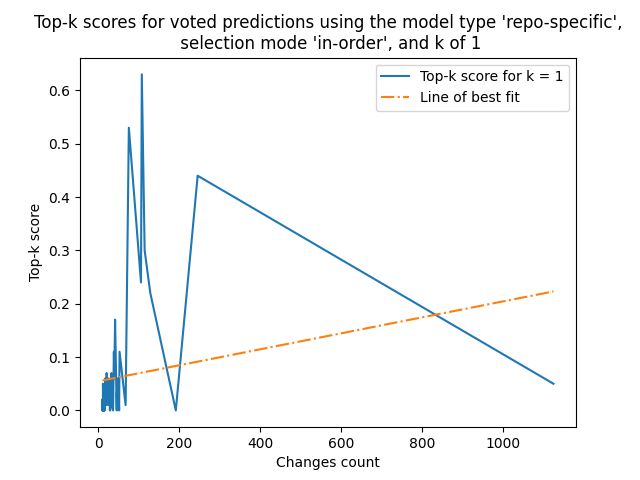
\includegraphics[height=5cm]{images/graphs/neural-network-top-k-voted-k-1-model-mode-repo-specific-selection-mode-in-order.png} }}%
    \subfloat[\centering Without mediawiki/core.]{{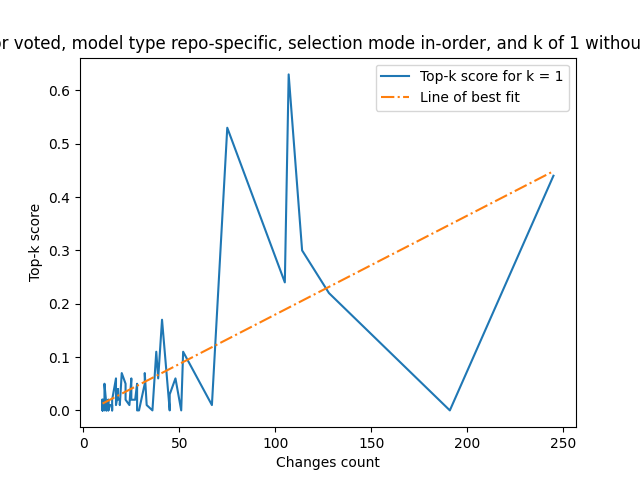
\includegraphics[height=5cm]{images/graphs/neural-network-top-k-voted-k-1-model-mode-repo-specific-selection-mode-in-order-no-core.png} }}%
    \caption{Neural network recommender Top-k score for correctly predicting voters where k is 1.}%
    \label{fig:neural-network-top-k-voted-k-1}%
\end{figure}

\begin{figure}[H]%
    \centering
    \subfloat[\centering All repositories.]{{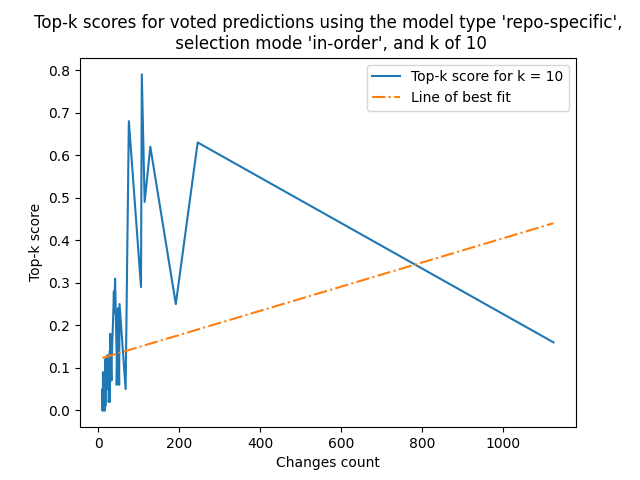
\includegraphics[height=5cm]{images/graphs/neural-network-top-k-voted-k-10-model-mode-repo-specific-selection-mode-in-order.png} }}%
    \subfloat[\centering Without mediawiki/core.]{{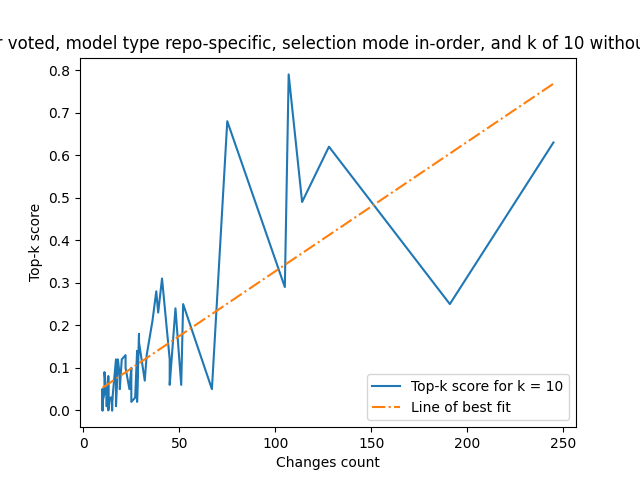
\includegraphics[height=5cm]{images/graphs/neural-network-top-k-voted-k-10-model-mode-repo-specific-selection-mode-in-order-no-core.png} }}%
    \caption{Neural network recommender Top-k score for correctly predicting voters where k is 10.}%
    \label{fig:neural-network-top-k-voted-k-10}%
\end{figure}

\begin{figure}[H]%
    \centering
    \subfloat[\centering All repositories selected for evaluation.]{{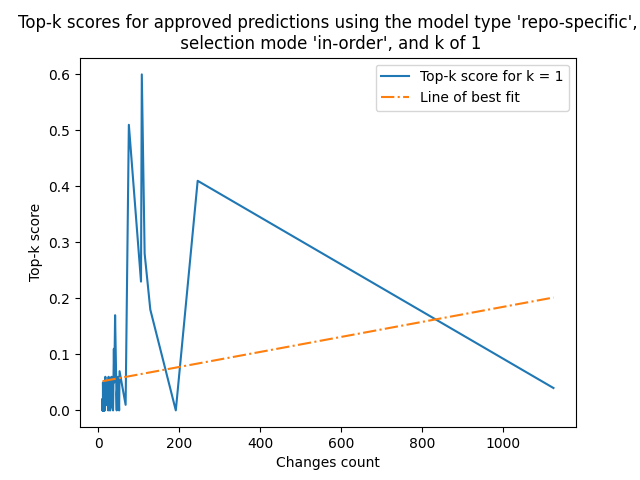
\includegraphics[height=5cm]{images/graphs/neural-network-top-k-approved-k-1-model-mode-repo-specific-selection-mode-in-order.png} }}%
    \subfloat[\centering Without mediawiki/core.]{{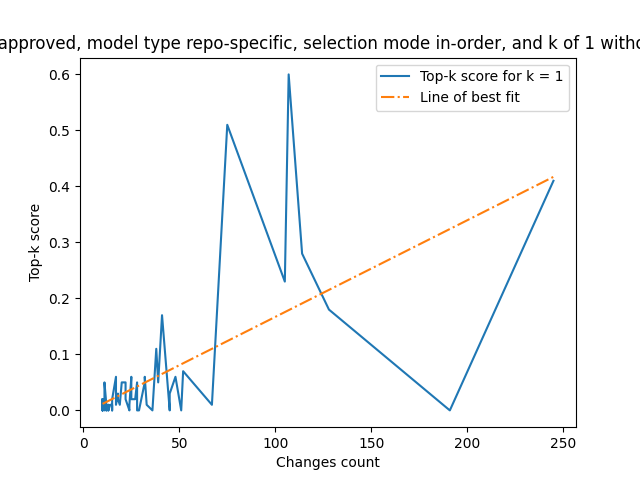
\includegraphics[height=5cm]{images/graphs/neural-network-top-k-approved-k-1-model-mode-repo-specific-selection-mode-in-order-no-core.png} }}%
    \caption{Neural network recommender Top-k score for correctly predicting approvers where k is 1.}%
    \label{fig:neural-network-top-k-approved-k-1}%
\end{figure}

\begin{figure}[H]%
    \centering
    \subfloat[\centering All repositories.]{{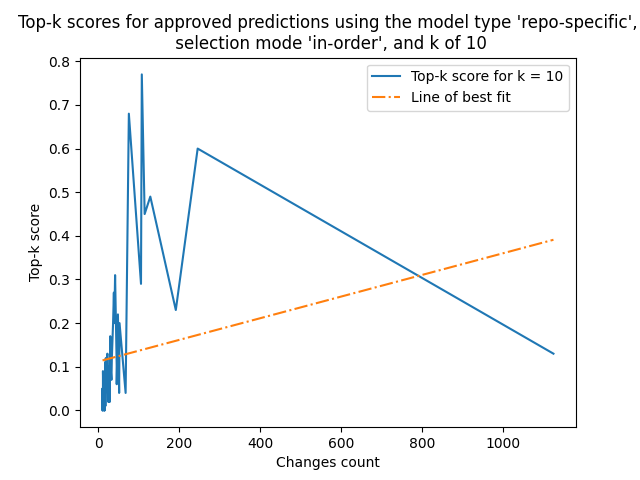
\includegraphics[height=5cm]{images/graphs/neural-network-top-k-approved-k-10-model-mode-repo-specific-selection-mode-in-order.png} }}%
    \subfloat[\centering Without mediawiki/core.]{{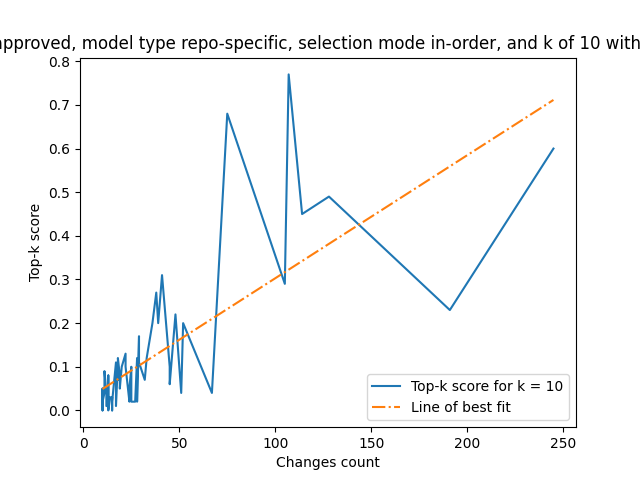
\includegraphics[height=5cm]{images/graphs/neural-network-top-k-approved-k-10-model-mode-repo-specific-selection-mode-in-order-no-core.png} }}%
    \caption{Neural network recommender Top-k score for correctly predicting approvers where k is 10.}%
    \label{fig:neural-network-top-k-approved-k-10}%
\end{figure}

To test whether the gradient in the graphs shown in Figures~\ref{fig:neural-network-top-k-voted-k-1}, \ref{fig:neural-network-top-k-voted-k-3-appendix-c}, \ref{fig:neural-network-top-k-voted-k-5-appendix-c}, and \ref{fig:neural-network-top-k-voted-k-10} are significant enough to indicate a relationship between the changes count (by extension the repository activity) and the Top-k score for predicting voters, the two-sided p-value is generated in the same way as was done when doing this for the rule based recommender. This data is detailed in Table~\ref{table:neural-network-top-k-line-of-best-fit-for-voted}

\begin{table}[H]
    \centering
    \begin{tabular}{@{}c c c c c@{}} 
    \hline
    \textbf{Graph label} & \textbf{K value} & \textbf{Gradient} & \textbf{Pearson correlation coefficient} & \textbf{two-sided p-value} \\
    \hline
Figure~\ref{fig:neural-network-top-k-approved-k-1} \emph{(a)} & 1 & 0.000134 & 0.166 & 0.201 \\
Figure~\ref{fig:neural-network-top-k-approved-k-1} \emph{(b)} & 1 & 0.00173 & 0.629 & 7.49e-08 \\
Figure~\ref{fig:neural-network-top-k-approved-k-3-appendix-c} \emph{(a)} & 3 & 0.000201 & 0.195 & 0.132 \\
Figure~\ref{fig:neural-network-top-k-approved-k-3-appendix-c} \emph{(b)} & 3 & 0.00255 & 0.73 & 3.56e-11 \\
Figure~\ref{fig:neural-network-top-k-approved-k-5-appendix-c} \emph{(a)} & 5 & 0.000215 & 0.201 & 0.121 \\
Figure~\ref{fig:neural-network-top-k-approved-k-5-appendix-c} \emph{(b)} & 5 & 0.00265 & 0.728 & 4.42e-11 \\
Figure~\ref{fig:neural-network-top-k-approved-k-10} \emph{(a)} & 10 & 0.000248 & 0.22 & 0.0883 \\
Figure~\ref{fig:neural-network-top-k-approved-k-10} \emph{(b)} & 10 & 0.00282 & 0.736 & 2.01e-11 \\
    \hline
    \end{tabular}
    \caption{Gradient, Pearson correlation coefficient and p-value for the line of best fit for graphs in Figures~\ref{fig:neural-network-top-k-approved-k-1}, \ref{fig:neural-network-top-k-approved-k-3-appendix-c}, \ref{fig:neural-network-top-k-approved-k-5-appendix-c}, and \ref{fig:neural-network-top-k-approved-k-10}.}
    \label{table:neural-network-top-k-line-of-best-fit-for-approved}
\end{table}

\begin{table}[H]
    \centering
    \begin{tabular}{@{}c c c c c@{}} 
    \hline
    \textbf{Graph label} & \textbf{K value} & \textbf{Gradient} & \textbf{Pearson correlation coefficient} & \textbf{two-sided p-value} \\
    \hline
Figure~\ref{fig:neural-network-top-k-voted-k-1} \emph{(a)} & 1 & 0.00015 & 0.176 & 0.176 \\
Figure~\ref{fig:neural-network-top-k-voted-k-1} \emph{(b)} & 1 & 0.00185 & 0.64 & 3.69e-08 \\
Figure~\ref{fig:neural-network-top-k-voted-k-3-appendix-c} \emph{(a)} & 3 & 0.000217 & 0.202 & 0.118 \\
Figure~\ref{fig:neural-network-top-k-voted-k-3-appendix-c} \emph{(b)} & 3 & 0.00272 & 0.747 & 7.24e-12 \\
Figure~\ref{fig:neural-network-top-k-voted-k-5-appendix-c} \emph{(a)} & 5 & 0.00023 & 0.206 & 0.112 \\
Figure~\ref{fig:neural-network-top-k-voted-k-5-appendix-c} \emph{(b)} & 5 & 0.00281 & 0.742 & 1.14e-11 \\
Figure~\ref{fig:neural-network-top-k-voted-k-10} \emph{(a)} & 10 & 0.000284 & 0.238 & 0.065 \\
Figure~\ref{fig:neural-network-top-k-voted-k-10} \emph{(b)} & 10 & 0.00304 & 0.75 & 5.47e-12 \\
    \hline
    \end{tabular}
    \caption{Gradient, Pearson correlation coefficient and p-value for the line of best fit for graphs in Figures~\ref{fig:neural-network-top-k-voted-k-1}, \ref{fig:neural-network-top-k-voted-k-3-appendix-c}, \ref{fig:neural-network-top-k-voted-k-5-appendix-c}, and \ref{fig:neural-network-top-k-voted-k-10}.}
    \label{table:neural-network-top-k-line-of-best-fit-for-voted}
\end{table}

The two-sided p-values in Tables~\ref{table:neural-network-top-k-line-of-best-fit-for-approved} and \ref{table:neural-network-top-k-line-of-best-fit-for-voted} are less than 0.05 if the graphs do not include mediawiki/core. For graphs including mediawiki/core the two-sided p-value does indicate enough significance to support a connection between the performance of the neural network model and change counts, and therefore \(H_0\) holds. When excluding mediawiki/core, there is enough evidence to reject \(H_0\) as the p-values are all zero with a pearson correlation coefficient greater than 0.5. This suggests that mediawiki/core is a statistically significant outlier and supports the assertion that for all repositories other than mediawiki/core the more active a repository is the better the neural network model is at predicting the right reviewers.

\section{Mean Reciprocal Rank (MRR)\label{section:evaluation-mrr}}

Both implementations were also evaluated using the Mean Reciprocal Rank (MRR). This method of evaluates the accuracy of the ranking of recommendations, where the user who voted/approved being closer to the top of the recommendations list causes a better score \citep[p. 506]{9240650}. While the MRR and Top-k score are similar, Top-k will only indicate that a user is recommended in the recommendations limited to the number k. For example, a good Top-k score where k is 10 could be made if the actual approver / voter is always in the 10th position, however, this would produce a poorer MRR score than if the actual reviewer / voter was ranked higher.

This method makes use of an equation shown in Equation~\ref{eq:mrr} that produces the MRR score and the equation used in this project is based on the equation detailed by \citeauthor{9240650} \citeyear{9240650} (p. 506). In this equation, like for Top-K, \(C\) is the list of changes and \(t\) represents either ``approved'' or ``voted''. The function \(rank(C(i), t)\) returns the position of the first voter or approver in the recommendations list generated for the \(i\)th change in \(C\). Whether the function looks for the first approver or first voter depends on the value provided in \(t\).

\begin{equation} \label{eq:mrr}
MRR(C, t) = \frac{1}{|C|} \sum_{i=0}^{|C|}\frac{1}{rank(C(i), t)}
\end{equation}

The \(rank(C(i), t)\) function for this project is approximated by the pusedo-code shown in Algorithm~\ref{alg:rank}. The function \(recommendations\_for\_change\) gets the recommendations for users who are expected to either vote or approve depending on the value in \(type\) for the \(change\). The result of \(MRR(C, t)\) is stored for later inspection.

\begin{algorithm}[H]
	\Fn{rank (change, type)} {
            $sanitised\_change \gets remove\_reviewer\_info\_from\_change$ $(change)$\;
            $recommendations \gets recommendations\_for\_change$ $(sanitised\_change, type)$\;
            \eIf{$type = voted$}{
                $actual\_reviewers \gets get\_actual\_voters$ $(change)$\;
            }{
                $actual\_reviewers \gets get\_actual\_approvers$ $(change)$\;
            }
            \ForEach{$\{recommendation\} \in recommendations$} {
                \If{$recommendation \in actual\_reviewers$} {
                    \Return $position\_of\_recommendation\_in\_recommendations\_list$ $(recommendation, recommendations)$\;
                }
            }
            \Return $|$recommendations$|$\;
	}
	\caption
	{\label{alg:rank}rank function.}
\end{algorithm}

\subsection{Rule Based Implementation}

For the rule based recommender, the MRR score was generated multiple times where each run had a unique combination of the following parameters to the function \(MRR(C, t)\):
\begin{itemize}
    \item \(t\) - The recommendation is asked to produce recommendations for users who would vote on the change or users who would approve the change.
    \item \(C\) - Changes for the repository split into ``merged'', ``open'' and ``abandoned'' changes.
\end{itemize}

The full MRR scores for the rule recommender can be found in Appendix~\ref{appendix:detailed-results}. \williamnote{Reference specific table, not the appendix?} A selection of these tabled results are shown in Table~\ref{table:rule-based-mrr-scores} with values over 0.4 highlighted for reference.

\begin{table}[H]
    \centering
    \begin{tabular}{@{}c c c@{}} 
 \hline
    \textbf{Repository} & \textbf{Approved} & \textbf{Voted} \\
\hline
mediawiki/extensions/CheckUser & 0.331 & 0.325 \\
mediawiki/extensions/SecureHTML & 0.0263 & 0.0351 \\
mediawiki/extensions/ShoutWikiAds & 0.0291 & 0.0291 \\
mediawiki/extensions/BlueSpiceInsertFile & 0.000575 & 0.000575 \\
mediawiki/extensions/MassMessage & 0.0448 & 0.0412 \\
mediawiki/extensions/Translate & 0.335 & 0.352 \\
mediawiki/extensions/CentralAuth & 0.0664 & 0.0664 \\
mediawiki/extensions/Workflows & 0.0341 & 0.0341 \\
mediawiki/core & 0.225 & 0.222 \\
mediawiki/extensions/GrowthExperiments & \textbf{0.546} & \textbf{0.568} \\
mediawiki/skins/Vector & 0.364 & 0.376 \\
\hline
\end{tabular}
    \caption{MRR scores for the rule based recommender implementation.}
    \label{table:rule-based-mrr-scores}
\end{table}

The MRR results suggest that the GrowthExperiments extension has users who actually approved or voted higher up the ranking than other repositories, whereas, the Translate extension may be recommending the actual reviewer/approver further down the list. These MRR results, like for Top-k, can be used to generate graphs against the number of changes in the testing and training dataset. The graphs in Figure~\ref{fig:rule-based-mrr-approved} shows the MRR scores when predicting users who would approve the change and Figure~\ref{fig:rule-based-mrr-voted} shows the MRR scores for predicting users who would vote on the change.

\williamnote{TODO: Ensure consistent capitalisation for top-k.}
\rcnote{I did this for the ones I encountered (using uppercase T).}

Like for Top-k, the graphs were produced for all repositories which are labelled \emph{(a)} and then for all repositories excluding ``mediawiki/core'' as the MRR score for that repository is also an outlier compared to the other scores.

\begin{figure}[H]%
    \centering
    \subfloat[\centering All repositories.]{{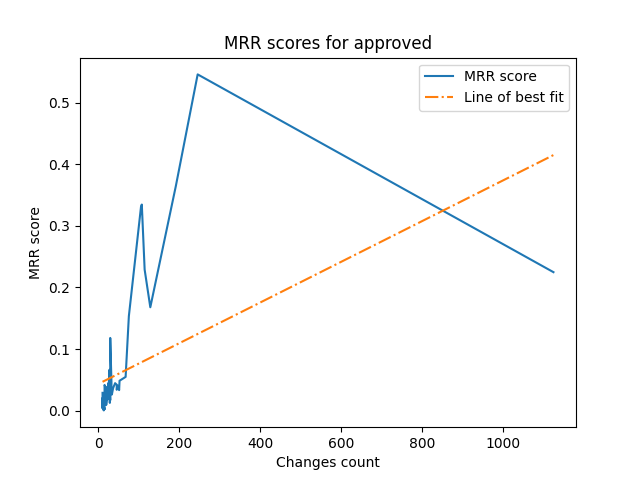
\includegraphics[height=5cm]{images/graphs/rule-based-mrr-approved.png} }}%
    \subfloat[\centering Without mediawiki/core.]{{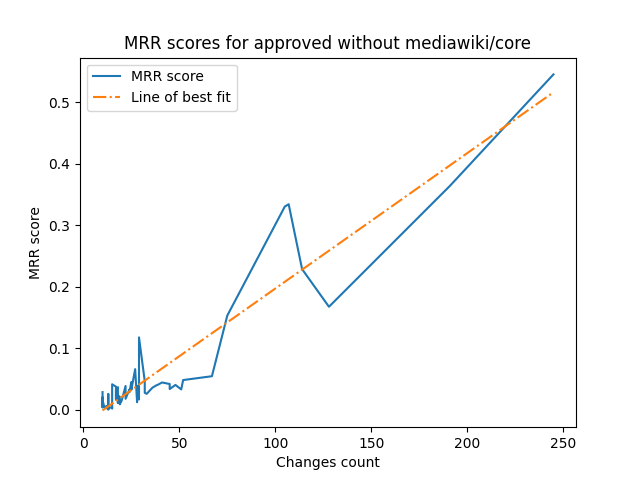
\includegraphics[height=5cm]{images/graphs/rule-based-mrr-approved-no-core.png} }}%
    \caption{Rule based recommender MRR score for correctly predicting approvers.}%
    \label{fig:rule-based-mrr-approved}%
\end{figure}

\begin{figure}[H]%
    \centering
    \subfloat[\centering All repositories.]{{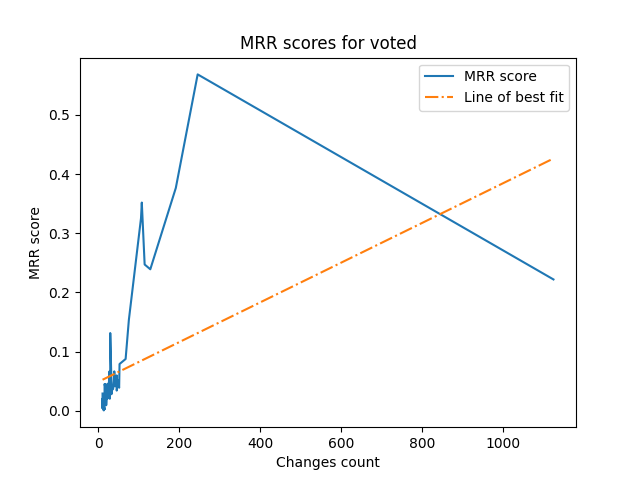
\includegraphics[height=5cm]{images/graphs/rule-based-mrr-voted.png} }}%
    \subfloat[\centering Without mediawiki/core.]{{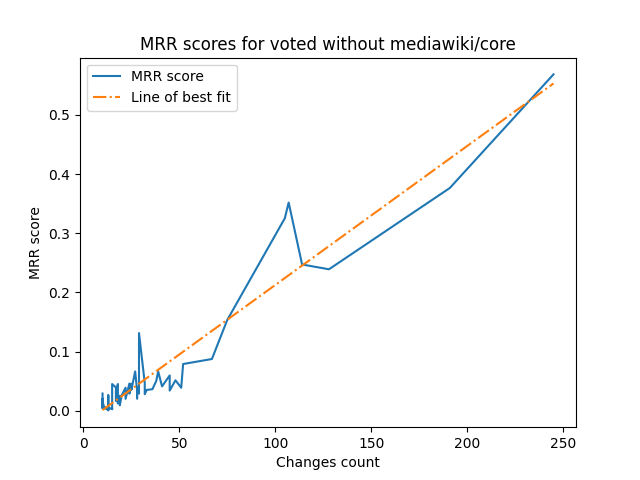
\includegraphics[height=5cm]{images/graphs/rule-based-mrr-voted-no-core.png} }}%
    \caption{Rule based recommender MRR score for correctly predicting voters.}%
    \label{fig:rule-based-mrr-voted}%
\end{figure}

The graphs, similarly to Top-k, produce a positive line of best fit. This is also analysed similarly to how the Top-k score line of best fit is analysed by using the pearson correaltion coefficent and the two-sided p-value.

\begin{table}[H]
    \centering
    \begin{tabular}{@{}c c c c c@{}} 
    \hline
    \textbf{Graph label} & \textbf{Gradient} & \textbf{Pearson correlation coefficient} & \textbf{two-sided p-value} \\
    \hline
Figure~\ref{fig:rule-based-mrr-approved} \emph{(a)} & 0.00033 & 0.468 & 0.000143 \\
Figure~\ref{fig:rule-based-mrr-approved} \emph{(b)} & 0.0022 & 0.939 & 1.49e-28 \\
Figure~\ref{fig:rule-based-mrr-voted} \emph{(a)} & 0.000336 & 0.456 & 0.000224 \\
Figure~\ref{fig:rule-based-mrr-voted} \emph{(b)} & 0.00235 & 0.956 & 1.53e-32 \\
    \hline
    \end{tabular}
    \caption{Gradient, Pearson correlation coefficient and p-value for the line of best fit for graphs in Figures~\ref{fig:rule-based-mrr-approved} and \ref{fig:rule-based-mrr-voted}.}
    \label{table:mrr-line-of-best-fit-stats}
\end{table}

The results in Table~\ref{table:mrr-line-of-best-fit-stats} support the assertion that when excluding mediawiki/core the number of changes causes a positive effect on the rule based recommendation accuracy. If including mediawiki/core, this is not clear enough to reject \(H_0\).

\subsection{Neural Network Implementation}

The MLP classifier implementation was also evaluated using the MRR metric. The MRR score was generated similarly to the rule based recommender, but for the selection mode of ``in-order'', changes limited to those which have been merged and model type of ``repo-specific'' were chosen. These were the settings used for neural network recommender to perform the Top-k analysis as discussed on page~\pageref{para:use-in-order-for-neural-network}. Choosing the same settings used for the Top-k evaluation is important as it allows the Top-k and MRR metric scores to be evaluated together when comparing to the rule based recommender and implementations in previous work in section~\ref{section:comparing-recommendations}.

The full MRR scores for the neural network recommender can be found in Appendix~\ref{appendix:detailed-results}. A selection of these tabled results are shown in Table~\ref{table:neural-network-mrr-scores}. The results in this table show that the Translate extension has a particularly good MRR score and beats the GrowthExperiments extension by a significant margin. This suggests that the neural network recommender recommends the actual approver/voter very near the top in the recommendations list.

\begin{table}[H]
    \centering
    \begin{tabular}{@{}c c c@{}} 
 \hline
    \textbf{Repository} & \textbf{Approved} & \textbf{Voted} \\
\hline
mediawiki/extensions/CheckUser & 0.255 & 0.263 \\
mediawiki/extensions/SecureHTML & 0.0588 & 0.0592 \\
mediawiki/extensions/ShoutWikiAds & 0.0205 & 0.0205 \\
mediawiki/extensions/BlueSpiceInsertFile & 0.0214 & 0.0214 \\
mediawiki/extensions/MassMessage & 0.224 & 0.226 \\
mediawiki/extensions/Translate & \textbf{0.707} & \textbf{0.751} \\
mediawiki/extensions/CentralAuth & 0.0225 & 0.0257 \\
mediawiki/core & 0.0734 & 0.0776 \\
mediawiki/extensions/GrowthExperiments & \textbf{0.502} & \textbf{0.532} \\
mediawiki/skins/Vector & 0.119 & 0.135 \\
\hline
\end{tabular}
    \caption{MRR scores for the neural network recommender implementation.}
    \label{table:neural-network-mrr-scores}
\end{table}

The MRR results for predicting users who vote and users who approve are graphed in Figures~\ref{fig:neural-network-mrr-approved} and \ref{fig:neural-network-mrr-voted}. Because mediawiki/core remains an outlier, the graphs are produced for all repositories used for the evaluation (labelled \emph{(a)}) and then for all repositories used for the evaluation except mediawiki/core (labelled \emph{(b)}). The graphs in these figures produce a line of best fit that is has a positive slope for all the graphs, but for the graphs including ``mediawiki/core'' this is substationally less steep.

\begin{figure}[H]%
    \centering
    \subfloat[\centering All repositories.]{{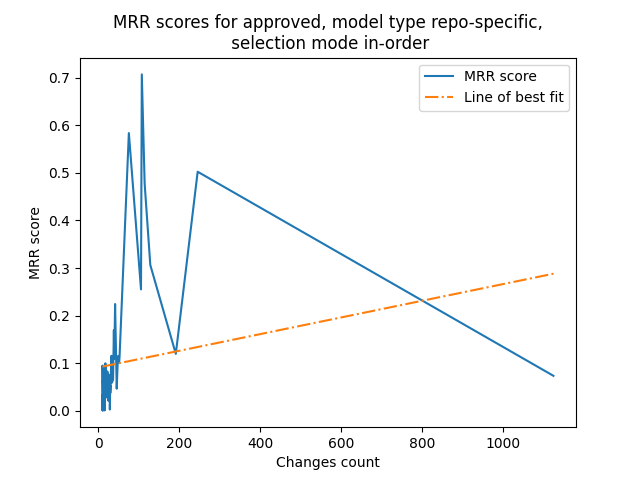
\includegraphics[height=5cm]{images/graphs/neural-network-mrr-approved-model-mode-repo-specific-selection-mode-in-order.png} }}%
    \subfloat[\centering Without mediawiki/core.]{{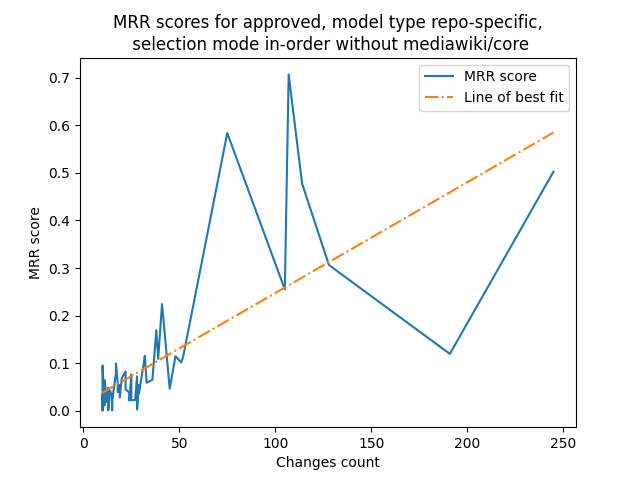
\includegraphics[height=5cm]{images/graphs/neural-network-mrr-approved-model-mode-repo-specific-selection-mode-in-order-no-core.png} }}%
    \caption{Neural network recommender MRR score for correctly predicting approvers.}%
    \label{fig:neural-network-mrr-approved}%
\end{figure}

\begin{figure}[H]%
    \centering
    \subfloat[\centering All repositories.]{{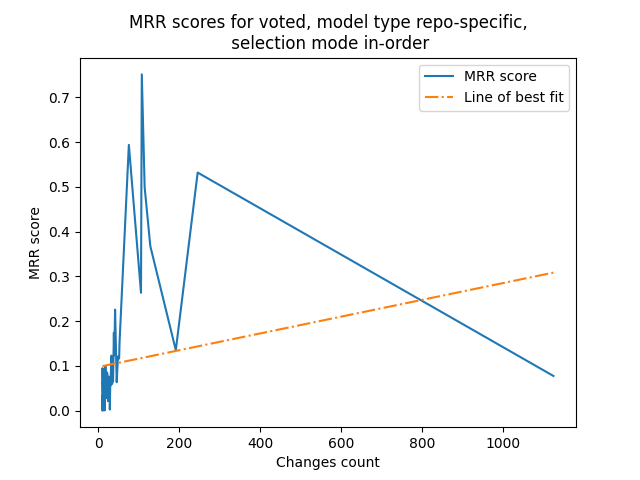
\includegraphics[height=5cm]{images/graphs/neural-network-mrr-voted-model-mode-repo-specific-selection-mode-in-order.png} }}%
    \subfloat[\centering Without mediawiki/core.]{{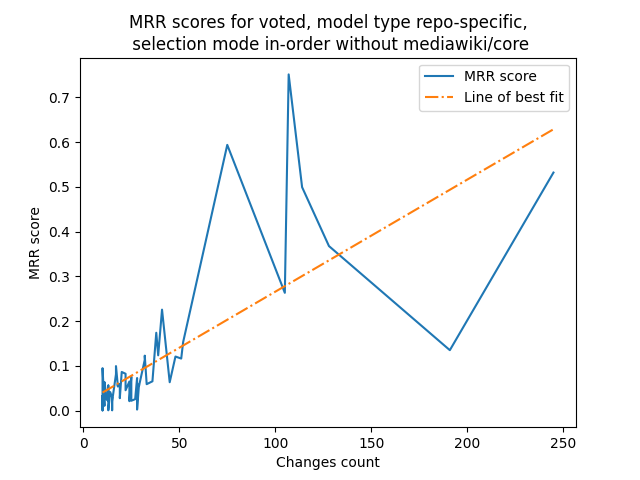
\includegraphics[height=5cm]{images/graphs/neural-network-mrr-voted-model-mode-repo-specific-selection-mode-in-order-no-core.png} }}%
    \caption{Neural network recommender MRR score for correctly predicting voters.}%
    \label{fig:neural-network-mrr-voted}%
\end{figure}

To quantify the relationship detailed in the line of best fit between the changes count in the testing and training data set and the MRR score, the Pearson correlation coefficient and two-sided p-value is produced which is shown in Table~\ref{table:mrr-line-of-best-fit-stats-neural-network}. These results show that when including ``mediawiki/core'' the line of best fit does not have a statistically significant enough line of best fit to reject \(H_0\). However, when excluding ``mediawiki/core'' the p-value is less than 0.05 and pearson correlation coefficent is greater than 0.5 which is enough evidence to accept \(H_1\). This is more evidence to suggest that ``mediawiki/core'' is an outlier.

\begin{table}[H]
    \centering
    \begin{tabular}{@{}c c c c c@{}} 
    \hline
    \textbf{Graph label} & \textbf{Gradient} & \textbf{Pearson correlation coefficient} & \textbf{two-sided p-value} \\
    \hline
Figure~\ref{fig:neural-network-mrr-approved} \emph{(a)} & 0.000175 & 0.183 & 0.174 \\
Figure~\ref{fig:neural-network-mrr-approved} \emph{(b)} & 0.00233 & 0.709 & 9.41e-10 \\
Figure~\ref{fig:neural-network-mrr-voted} \emph{(a)} & 0.000187 & 0.186 & 0.167 \\
Figure~\ref{fig:neural-network-mrr-voted} \emph{(b)} & 0.0025 & 0.724 & 2.87e-10 \\
    \hline
    \end{tabular}
    \caption{Gradient, Pearson correlation coefficient and two-sided p-value for the line of best fit for graphs in Figures~\ref{fig:neural-network-mrr-approved} and \ref{fig:neural-network-mrr-voted}.}
    \label{table:mrr-line-of-best-fit-stats-neural-network}
\end{table}


\section{Accuracy Score\label{section:accuracy-score}}
The MLP classifier recommender was trained using a randomly sampled selection of the testing and training data. The other part not selected for training was used to test the created models. The first metric used to evaluate is the \emph{sklearn}'s accuracy\_score which produces an accuracy score for the classifications produced by the model \citep{sklearn:accuracy-score}. In this project's case the values returned are normalised between 1 and 0, which is \enquote{the fraction of correctly classified samples} \citep{sklearn:accuracy-score}. This means that the accuracy score being closer to 1 indicates a better model, though even if the accuracy score is close to 1 the model could be predicting that no one would vote or merge a change.

As with the other metrics the the results from all evaluated repositories are in Appendix~\ref{appendix:detailed-results}. The same repositories used to highlight the results in the Top-k and MRR evaluation sections have been chosen to be shown here. Table~\ref{table:accuracy-score-average} shows the average accuracy score for these repositories. The accuracy scores shown in the table vary widely per repository, and for the CheckUser extension the accuracy is very high for predicting approvers but very poor for predicting voters.

\begin{table}[H]
    \centering
    \begin{tabular}{@{}c c c@{}} 
    \hline
    \textbf{Repository} & \multicolumn{2}{c}{\textbf{Accuracy score}} \\
    & \textbf{Approved} & \textbf{Voted} \\
\hline
mediawiki/extensions/BlueSpiceInsertFile & 0.972 & 0.978 \\
mediawiki/extensions/CentralAuth & 0.188 & 0.781 \\
mediawiki/extensions/CheckUser & 0.99 & 0.084 \\
mediawiki/extensions/GrowthExperiments & 0.116 & 0.889 \\
mediawiki/extensions/MassMessage & 0.985 & 0.949 \\
mediawiki/extensions/SecureHTML & 0.99 & 0.985 \\
mediawiki/extensions/ShoutWikiAds & 0.958 & 0.958 \\
mediawiki/extensions/Translate & 0.989 & 0.98 \\
mediawiki/extensions/Workflows & 0.992 & 0.992 \\
mediawiki/core & 0.461 & 0.542 \\
mediawiki/skins/Vector & 0.144 & 0.877 \\
    \hline
    \end{tabular}
    \caption{Average accuracy score for predicting users who voted and approved.}
    \label{table:accuracy-score-average}
\end{table}

When graphing of number of changes against accuracy score for the repo-specific models as shown in Figure~\ref{fig:accuracy-score-average-graphed} it is clear that the number of changes in the training and testing data set have no effect on the accuracy score. \williamnote{TOOD: Why is this the case?}

\begin{figure}[h]
    \centering
    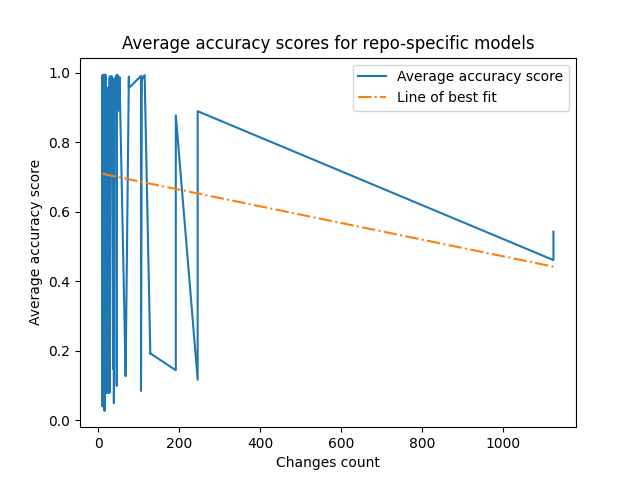
\includegraphics[scale=0.5]{images/graphs/neural-network-avg-accuracy-repo-specific.png}
    \caption{Change counts in the training and testing data set against average accuracy score}
    \label{fig:accuracy-score-average-graphed}
\end{figure}

\section{Confusion Matrix\label{section:confusion-matrix}}
The MLP classifier implementation was also tested using \emph{sklearn}'s confusion\_matrix which produces a confusion matrix for classification models \citep{sklearn:confusion-matrix}. This matrix holds values as described in Matrix~\ref{matrix:confusion-matrix}.

\begin{equation}
\begin{bmatrix}
$True negatives$ & $False negatives$ \\
$False positives$ & $True positives$
\end{bmatrix}
\label{matrix:confusion-matrix}
\end{equation}
\hspace{0.25cm}

A model with a good accuracy score may be good at predicting that no one will vote or approve a change and therefore, the confusion matrix can be used to monitor the number of predictions that a user would vote or approve.

In the case of this project, a good confusion matrix will minimise false positives while ensuring that there are enough true positives. This is because recommending users who are not appropriate for the change would lead to ineffective recommendations, however, still ensuring that there are enough `positives' is needed so that recommendations can be split between a larger group to avoid overloading a particular user with review requests.

The number of results generated for this metric means that Appendix~\ref{appendix:detailed-results} does not contain tables for these results as it would cause the appendix to be too large. However, these results are available in full in the results JSON file in the code for this project.

The extensions Translate and GrowthExperiments are chosen for evaluation here. The Translate extension received accuracy scores of \(0.989\) and \(0.98\) as shown in Table~\ref{table:accuracy-score-average} which could be because the model is predicting very few reviewers. GrowthExperiments is chosen as it has accuracy scores of \(0.116\) and \(0.889\) for predicting approvers and voters respectively. This difference may be explained in the confusion matrix for the approvers and voters.

As can be seen in Equation~\ref{matrix:confusion-matrix-voted-translate} and \ref{matrix:confusion-matrix-approved-translate}, the model predicts that on average 3.963 users have voted and 1.296 have approved. The predicted number of approvers being close to 1 is a good sign as usually only one user will give an approval vote to a change. The confusion matrices suggest that the repo-specific model for the Translate extension predicts relatively well and doesn't seem to have the issue of predicting all users will not vote or approve.

\begin{figure}[H]
\begin{equation}
\begin{bmatrix}
$170.630$ & $0.370$ \\
$3.074$ & $0.889$
\end{bmatrix}
\label{matrix:confusion-matrix-voted-translate}
\end{equation}
\\{Average confusion matrix values for the Translate extension when predicting voters}
\end{figure}
\hspace{0.25cm}

\begin{figure}[H]
\begin{equation}
\begin{bmatrix}
$172.815$ & $0.852$ \\
$1.111$ & $0.185$
\end{bmatrix}
\label{matrix:confusion-matrix-approved-translate}
\end{equation}
\\{Average confusion matrix values for the Translate extension when predicting approvers}
\end{figure}
\hspace{0.25cm}

As can be seen in Equation~\ref{matrix:confusion-matrix-voted-growth} and \ref{matrix:confusion-matrix-approved-growth}, the model predicts that on average 18.387 users have voted and 143.629 have approved. This is in stark contrast to the confusion matrices for the Translate extension. As such this confusion matrix strongly suggests that the repo-specific model is not trained well for the approval vote type and for the prediction of voters the model is not particularly good.

\begin{figure}[H]
\begin{equation}
\begin{bmatrix}
$143.113$ & $0.565$ \\
$17.597$ & $0.790$
\end{bmatrix}
\label{matrix:confusion-matrix-voted-growth}
\end{equation}
\\{Average confusion matrix values for the GrowthExperiments extension when predicting voters}
\end{figure}
\hspace{0.25cm}

\begin{figure}[H]
\begin{equation}
\begin{bmatrix}
$18.226$ & $0.210$ \\
$142.839$ & $0.790$
\end{bmatrix}
\label{matrix:confusion-matrix-approved-growth}
\end{equation}
\\{Average confusion matrix values for the GrowthExperiments extension when predicting approvers}
\end{figure}
\hspace{0.25cm}

\section{Perceived accuracy of recommendations\label{section:perceived-accuracy-of-recommendations}}
To provide some non-statistical methods of evaluation, a select few example changes were chosen and both implementations were asked to produce recommendations. This was done so that we could
\begin{itemize}
    \item See whether recommendations were being appropriately de-duplicated
    \item Compare the recommendations to the reviewers on the change and who voted/approved the change if the change has votes
    \item Allow comparison to occur against the ReviewerBot by comparing the users it adds to the change with the recommendations produced.
    \item Provide screenshots of the implementations running for this project
\end{itemize}

Both changes that were selected were uploaded by the author of this report. This is done so that the author has a good idea about who would be best to review as this method is highly subjective. In Figure~\ref{fig:checkuser-example-change-1} the web-page on the Gerrit system for the first selected change is shown. This change is on the CheckUser extension repository and has been merged. Figure~\ref{fig:rule-based-recommender-result-for-example-change-1} shows the recommendations produced for this change by the rule based recommender and Figure~\ref{fig:neural-network-recommender-result-for-example-change-1} shows recommendations produced by the neural network implementation.

\begin{figure}[H]
    \centering
    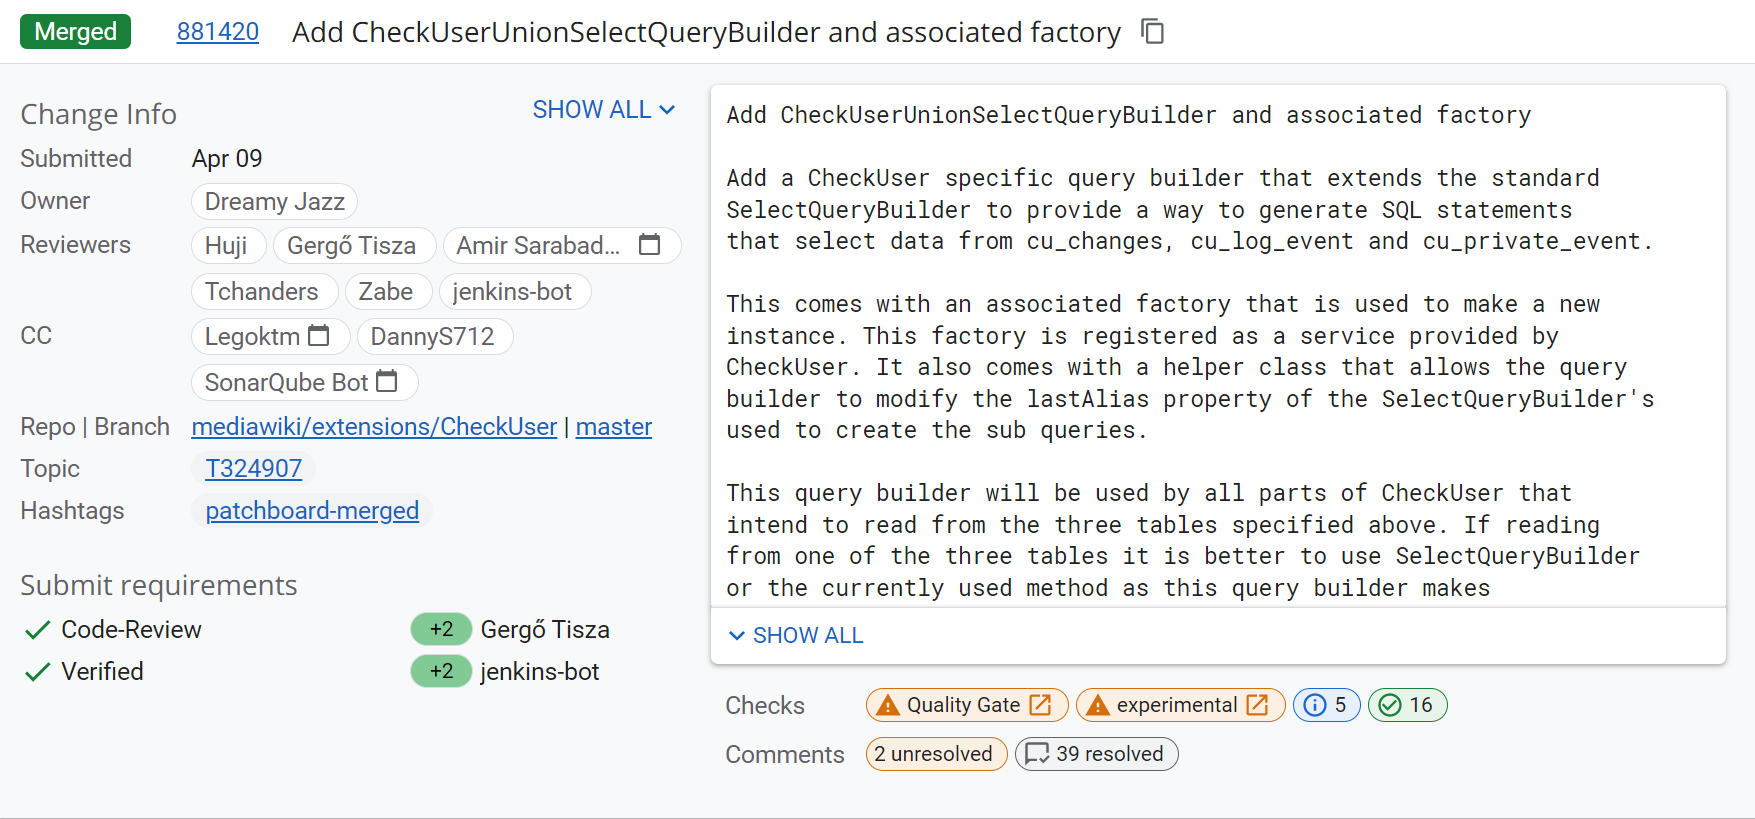
\includegraphics[scale=0.6]{images/checkuser-example-change-1-on-gerrit.png}
    \caption{First change used for evaluating the accuracy of recommendations that comes from the CheckUser extension and is merged.}
    \label{fig:checkuser-example-change-1}
\end{figure}

\begin{figure}[H]
    \centering
    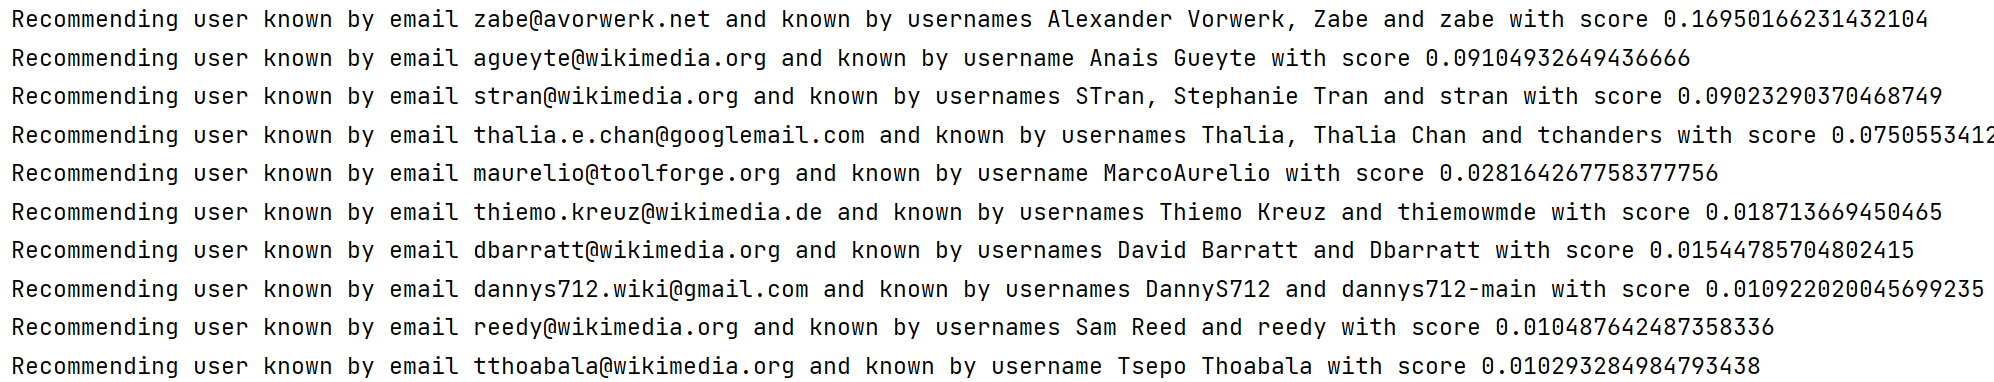
\includegraphics[scale=0.5]{images/rule-based-example-1.png}
    \caption{Recommendations produced by the rule based recommender for the first example change}
    \label{fig:rule-based-recommender-result-for-example-change-1}
\end{figure}

\begin{figure}[H]
    \centering
    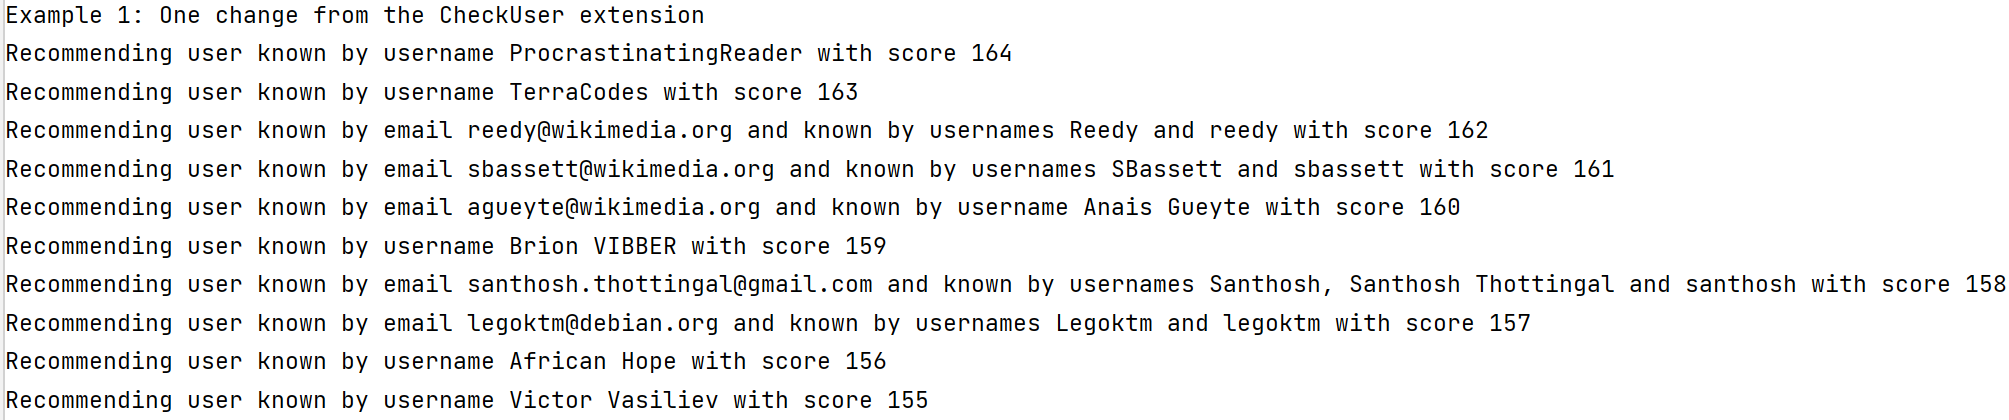
\includegraphics[scale=0.5]{images/neural-network-example-1.png}
    \caption{Recommendations produced by the neural network recommender for the first example change}
    \label{fig:neural-network-recommender-result-for-example-change-1}
\end{figure}

The recommendations produced in Figure~\ref{fig:rule-based-recommender-result-for-example-change-1} are very good. Out of 10 recommendations, three users recommended were already on the change as reviewers or users copied in. The first recommendation of Zabe was a good one as this user has reviewed many changes for the CheckUser extension. The users recommended positions 2, 3, 4 and 10 are staff members of the Wikimedia Foundation software development team that are responsible for this extension. The recommendations produced in Figure~\ref{fig:neural-network-recommender-result-for-example-change-1} are not nearly as good. The only recommendations that we see as particularly useful are the third (Reedy), fifth (Anais Gueyte) and eighth (Legoktm).

In Figure~\ref{fig:massmessage-example-change} the web-page on the Gerrit system for the second selected change is shown that is from the MassMessage extension and is currently open (though marked as work in progress). Figure~\ref{fig:rule-based-recommender-result-for-example-change-2} shows the recommendations produced for this change by the rule based recommender and Figure~\ref{fig:neural-network-recommender-result-for-example-change-2} shows recommendations produced by the neural network implementation.

\begin{figure}[H]
    \centering
    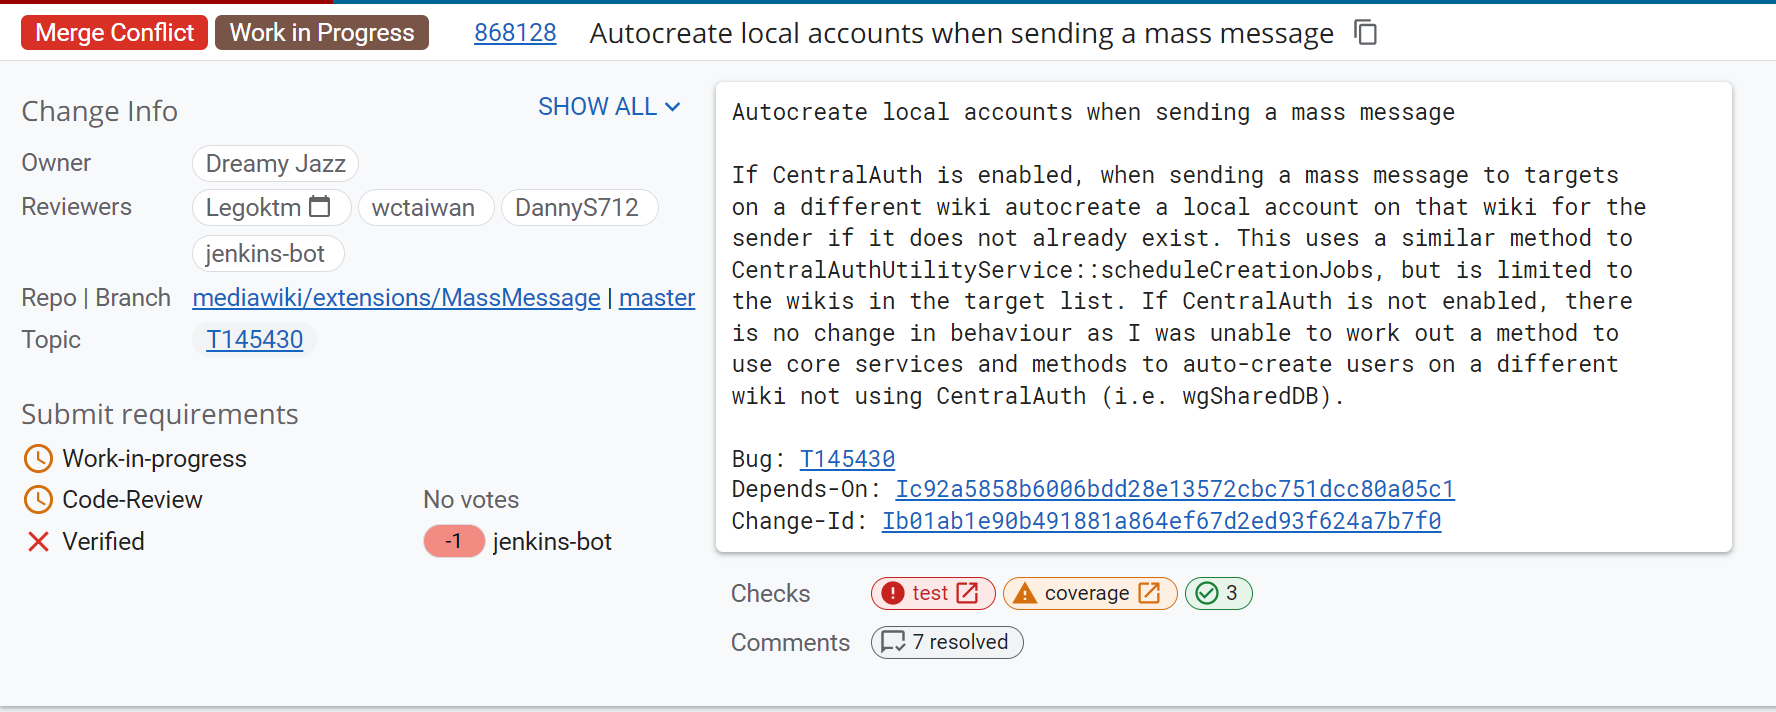
\includegraphics[scale=0.6]{images/massmessage-example-change-2.png}
    \caption{Second change used for evaluating the accuracy of recommendations that comes from the MassMessage extension and is open but work in progress and merge conflicts.}
    \label{fig:massmessage-example-change}
\end{figure}

\begin{figure}[H]
    \centering
    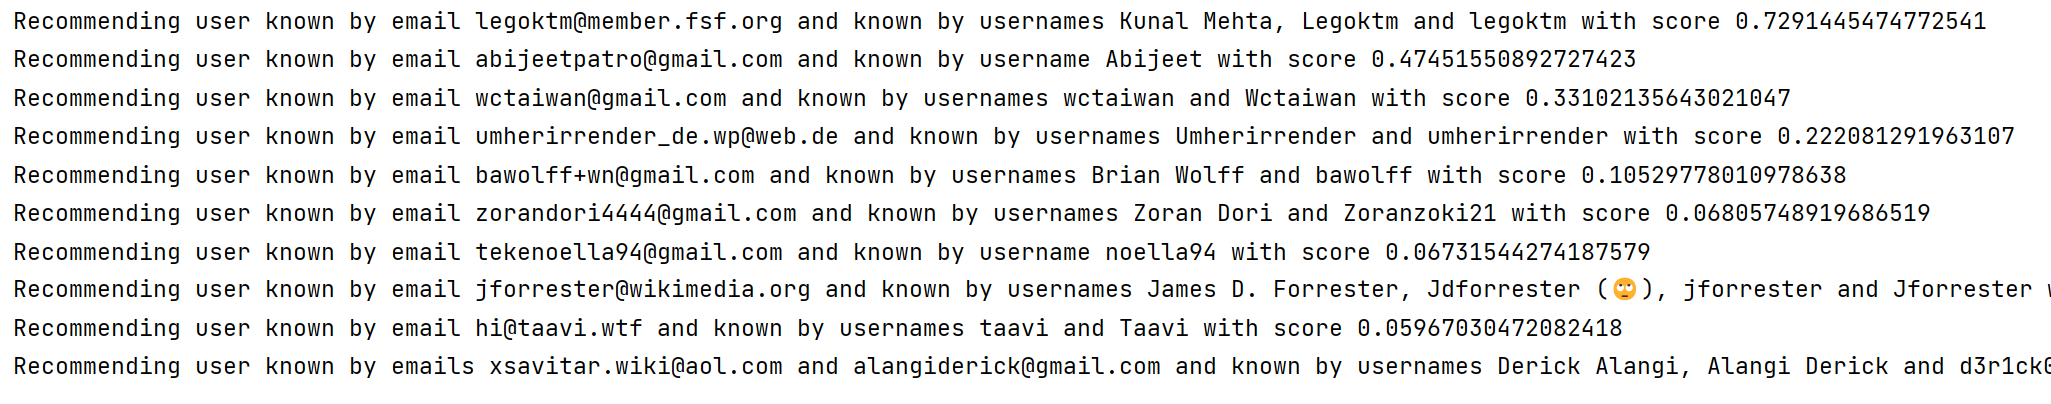
\includegraphics[scale=0.5]{images/rule-based-recommender-example-2.png}
    \caption{Recommendations produced by the rule based recommender for the second example change}
    \label{fig:rule-based-recommender-result-for-example-change-2}
\end{figure}

\begin{figure}[H]
    \centering
    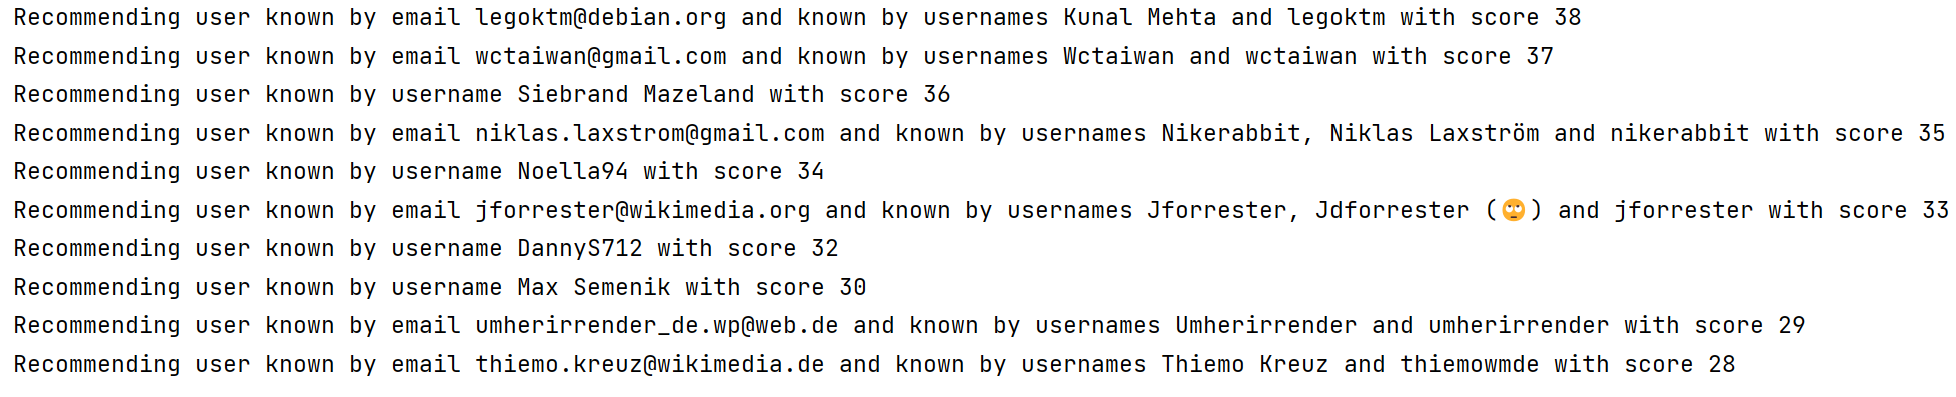
\includegraphics[scale=0.55]{images/neural-network-example-2.png}
    \caption{Recommendations produced by the neural network recommender for the second example change}
    \label{fig:neural-network-recommender-result-for-example-change-2}
\end{figure}

The recommendations produced by the rule recommender in Figure~\ref{fig:rule-based-recommender-result-for-example-change-2} are very good. The first and third recommendation are for users who are marked as the authors of this extension on the MediaWiki page for the extension \citepmediawiki{mediawiki:mass-message}. The other recommendations seem sensible, though there isn't as clear of a way to detail why. The recommendations produced by the neural network recommender in Figure~\ref{fig:neural-network-recommender-result-for-example-change-2} are about equivalent, and in some ways better. The two listed authors of the extension are the first two recommendations, which is better than first and third. Most of the other recommendations also make sense based on knowledge of these users.

As part of the analysis using this method it was discovered that some users with rights to merge code were not collected. This is because some users were granted access to the ``mediawiki'' group implicitly by being in the ``wmf'' group on another system known as ``LDAP'' \citep{wikitech:ldap-wmf}. This data could not be collected and used for this project, as it would have required re-training the neural network recommender and performing the evaluation for both implementations again. Doing that would have taken several days to complete at least, which was not possible. Including these users could be part of future work as discussed in section~\ref{section:future-work}.

\section{Comparing Implementations\label{section:comparing-recommendations}}

Using the evaluation metrics that were discussed at the start of this chapter, we now use these to compare our two implementations:
\begin{itemize}
    \item Against each other
    \item Against previous research
    \item Against the in-use ReviewerBot system
\end{itemize}

The comparisons of the implementations against each other are done by comparing the Top-k and MRR metric scores. A higher MRR and/or Top-k score indicates that the implementation performs better. The perceived accuracy of recommendations is also taken into account, though not relied on as heavily due to the method being more subjective.

The Top-k and MRR scores detailed in several implementations proposed in previous research are compared against the Top-k and MRR scores found in this chapter for the two implementations. A higher MRR and/or Top-k score would indicate that the implementation in question performs better.

Finally, the implementations proposed in this report are compared against the existing ReviewerBot system by comparing the recommendations against those who would be added by the bot to the change. This is done to evaluate whether the implementations provide any benefit over the existing system, as if there is no extra benefit this system would not be used on the \emph{live} MediaWiki Gerrit system.

\williamnote{TODO: Ensure consistent capitalisation in section titles.}

\subsection{Rule based vs Neural network\label{section:rule-based-against-neural-network}}

A comparison of the Top-k scores between the rule based recommender (detailed in Tables~\ref{table:top-k-approved} and \ref{table:top-k-voted}) and neural network recommender (detailed in Tables~\ref{table:top-k-approved-neural-network} and \ref{table:top-k-voted-neural-network}) suggests that in general the rule based recommender produces a better Top-k score and therefore better recommendations. However, for the repository ``mediawiki/extensions/Translate'' this is reversed as the Top-k score is better for the neural network recommender.

Comparing the MRR scores between the rule based recommender (detailed in Table~\ref{table:rule-based-mrr-scores}) and neural network recommender (detailed in Table~\ref{table:neural-network-mrr-scores}), the results are similar to the Top-k comparison where the rule based recommender performs better on most repositories with an exception of ``mediawiki/extensions/Translate'' which performs substantially better with the voted MRR result increasing by \(0.399\) and the approved MRR result increasing by \(0.372\).

When comparing the recommendations in section~\ref{section:perceived-accuracy-of-recommendations}, the rule based implementation was generally better at producing recommendations. For the second change, both implementations were similar but the first change had the neural network recommender produce significantly worse recommendations.

As such, the overall better Top-k and MRR metrics indicate that the rule based recommender is generally a better option. However, for specific repositories the neural network recommender may produce better recommendations and if further adjustments are made in future work to both implementations the balance may change.

If only one implementation could be used on the \emph{live} MediaWiki Gerrit system, the rule based recommender would be the most obvious choice unless the neural network recommender is improved and provides much better recommendations. This is because:
\begin{itemize}
    \item The process of input data to recommended users is clearly visible, unlike the neural network method that makes the transformation of input data to classification fairly opaque.
    \item The modification of the importance of any input data type can be done by just modifying numbers in a JSON file and does not require the re-training of the implementation. As such changes can be made on the fly and using any text editor.
\end{itemize}

To reduce the issues surrounding only recommending a few specific users, the rule based recommender could be extended to apply the ``semi-random'' selection mode to the recommendations so that it produces a list that doesn't always recommend one or two users, but instead picks from the top 5 to be the most recommended. In active enough repositories this semi-random selection should not cause too many issues, as any one of those top 5 reviewers should be able to review the change.

\subsection{Other Implementations\label{section:other-implementations-comparisons}}

Overall the rule based implementation performs slightly worse compared to implementations in previous research. This is because the two metrics, Top-k and MRR, usually have smaller or similar values compared to the three implementations detailed in \cite{9240650} (p. 507), where two of these are from \cite{7081824} and \cite{7332472}. 

However, for the GrowthExperiments extension the Top-1 score for predicting voters of \(0.44\) from Table~\ref{table:top-k-approved} and the Top-1 score for predicting approvers of \(0.393\) is better than any Top-1 score detailed by \cite{9240650}, \cite{7081824}, or \cite{7332472} as found by the table in \cite{9240650} (p. 507). For other values of k, the GrowthExperiments extension has similar Top-k scores to the implementation proposed by \cite{9240650} which is named ``recommended system'' (RS for short) and is slightly worse overall compared to other implementations. The MRR score for predicting both voters and approvers of \(0.546\) and \(0.568\) is better than any MRR score for the implementation named RS proposed in \cite{9240650}.

This means that with some further modification of the weights for the rule based recommender, the system could perform better than previous research. To achieve this effectively using per-repository weights may be needed.

Because the neural network recommender performs worse than the rule based recommender, it also performs worse compared to previous research in \cite{9240650}, \cite{7081824}, or \cite{7332472}. However, like the rule based recommender particular repositories had particularly good Top-k and MRR scores. In this case the GrowthExperiments and Translate were particularly good, with Top-1 scores for predicting both approvers and voters outperforming any Top-1 score for \cite{9240650}, \cite{7081824}, or \cite{7332472}. The MRR score for predicting voters or approvers is also generally worse, except for the GrowthExperiments and Translate extensions which either have similar or better MRR scores. The Translate extension MRR scores of \(0.707\) for predicting approvers and \(0.751\) predicting voters is better than every other MRR score detailed in \cite{9240650}, \cite{7081824}, or \cite{7332472} except for one from \cite{7332472} of \(0.84\).

As such the neural network needs further modification to perform as well as previous work, but specific repositories show that this implementation does work in some cases better than previous implementations and could work overall better if future research improved on the work carried out here.

\subsection{Benefits over ReviewerBot}

Using the example changes evaluated in section~\ref{section:perceived-accuracy-of-recommendations} the implementations proposed in this report are compared against the existing ReviewerBot system that uses the Git reviewers list\footnote{\url{https://www.mediawiki.org/w/index.php?title=Git/Reviewers\&oldid=5899016}. Accessed 3 May 2023} to add users who ask to be added to changes for specific repositories.

The Git reviewers list for the CheckUser extension is shown in Figure~\ref{fig:checkuser-extension-reviewer-list-for-evaluation}\footnote{This was previously shown in Chapter~\ref{chap:background-and-related-work} as Figure~\ref{fig:checkuser-extension-reviewer-list} but was included here again to make it easy to reference.}. One of the users on this list, Dreamy Jazz, is not recommended because they created the change used as the example.

\begin{figure}[h]
    \centering
    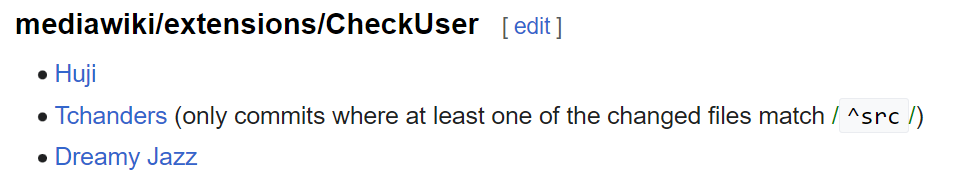
\includegraphics[scale=0.9]{images/git-reviewers-list-checkuser.png}
    \caption[Git reviewers list for the CheckUser extension.]{Git reviewers list for the CheckUser extension. Image credit: Screenshot of the page \url{https://www.mediawiki.org/wiki/Git/Reviewers\#mediawiki/extensions/CheckUser}. Accessed 30 April 2023.}
    \label{fig:checkuser-extension-reviewer-list-for-evaluation}
\end{figure}

The rule based recommender recommended well for the first change. The top 5 recommendations made sense and would be people who I would consider good users to review a change on this repository. Only one of these 5 users is on the Git reviewers list (Tchanders) and therefore these 4 other users would be not be considered as potential reviewers for the change.

The neural network recommender produced poor recommendations for this first change, however, two of the users recommended in the recommendations would be potentially useful on the change. One of these (Legoktm) has been added on the change as ``cc'' which means they are sent notifications about the change but not marked as one of the reviewers \citep{gerrit:cc-meaning}.

The second change was to the MassMessage extension which has two users in the Git reviewers list as shown in Figure~\ref{fig:massmessage-extension-reviewer-list}.

\begin{figure}[h]
    \centering
    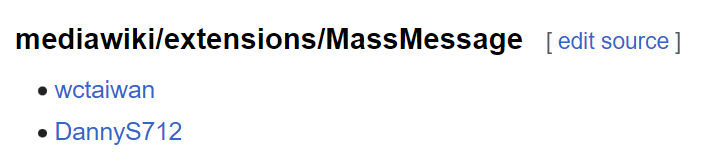
\includegraphics[scale=0.9]{images/git-reviewers-list-massmessage.png}
    \caption[Git reviewers list for the MassMessage extension.]{Git reviewers list for the CheckUser extension. Image credit: Screenshot of the page \url{https://www.mediawiki.org/wiki/Git/Reviewers\#mediawiki/extensions/MassMessage}. Accessed 30 April 2023.}
    \label{fig:massmessage-extension-reviewer-list}
\end{figure}

The recommendations produced by the rule based recommender for the second change were also good. The first and third as mentioned in section~\ref{section:perceived-accuracy-of-recommendations} were the authors of the extension. The first recommendation for Legoktm is not on the Git reviewers list, so the system would be able to suggest this user. Other users in the recommendations list for this change would be good too and are not on the Git reviewers list.

Recommendations from the neural network recommender for the second change were also fairly good. Again the user Legoktm is recommended who isn't on the Git reviewers list, while both users on the Git reviewers list are also present in the recommendations.